%\documentclass{fast-nuces-bs}
\documentclass[12pt,a4paper]{article}

\usepackage{blindtext}
\usepackage{mathptmx}% Times Roman font
\usepackage[T1]{fontenc}
\usepackage{lipsum} 
\usepackage{sectsty}
\usepackage{titlesec}
\usepackage{graphicx}
\usepackage{float}
\usepackage{tikz}
\usetikzlibrary{shapes,arrows,positioning,fit,calc,decorations.pathmorphing,shapes.geometric}
\usepackage{pgfplots}
\usepackage{listings}
\usepackage{xcolor}
\usepackage[hidelinks,colorlinks=false]{hyperref}
\usepackage{amsmath}
\usepackage{algorithm}
\usepackage{algorithmic}
\usepackage{booktabs}  % Professional table styling
\usepackage{array}     % Enhanced array support
\usepackage{tabularx}  % Extended tabular
\usepackage{longtable} % Multi-page tables

% Code listing configuration
\lstset{
    language=Python,
    basicstyle=\ttfamily\small,
    keywordstyle=\color{blue}\bfseries,
    commentstyle=\color{green!60!black},
    stringstyle=\color{red},
    numbers=left,
    numberstyle=\tiny\color{gray},
    stepnumber=1,
    numbersep=5pt,
    backgroundcolor=\color{gray!10},
    frame=single,
    breaklines=true,
    breakatwhitespace=true,
    tabsize=4,
    showstringspaces=false
}

% Custom commands for thesis information
\newcommand{\department}[1]{\gdef\@department{#1}}
\newcommand{\faculty}[1]{\gdef\@faculty{#1}}
\newcommand{\degreeyear}[1]{\gdef\@degreeyear{#1}}
\newcommand{\degreemonth}[1]{\gdef\@degreemonth{#1}}
\newcommand{\degreename}[1]{\gdef\@degreename{#1}}
\newcommand{\campuscity}[1]{\gdef\@campuscity{#1}}
\newcommand{\authorone}[2]{\gdef\@authorone{#1}\gdef\@authoroneroll{#2}}
\newcommand{\authortwo}[2]{\gdef\@authortwo{#1}\gdef\@authortworoll{#2}}
\newcommand{\authorthree}[2]{\gdef\@authorthree{#1}\gdef\@authorthreeroll{#2}}
\newcommand{\supervisor}[1]{\gdef\@supervisor{#1}}
\newcommand{\sessionduration}[1]{\gdef\@sessionduration{#1}}
\newcommand{\cosupervisor}[1]{\gdef\@cosupervisor{#1}}
\newcommand{\deanname}[1]{\gdef\@deanname{#1}}
\newcommand{\directorname}[1]{\gdef\@directorname{#1}}
\newcommand{\hodname}[1]{\gdef\@hodname{#1}}
\newcommand{\fypcoordinatorname}[1]{\gdef\@fypcoordinatorname{#1}}

% Set default values
\department{Department of Computer Science}
\faculty{Computer Science}
\degreeyear{2024}
\degreemonth{June}
\degreename{Software Engineering}
\campuscity{Islamabad}
\authorone{Abdur Rafae}{22i-2638}
\authortwo{Muneb Kazmi}{22i-2680}
\authorthree{Ahmed Javed}{22i-2461}
\supervisor{Ms. Rabail Zhid}
\sessionduration{2020-2024}
\cosupervisor{}
\deanname{Dr. Dean Computing}
\directorname{Dr. Director of the Campus}
\hodname{Dr. Head of Computer Science Department}
\fypcoordinatorname{Name of FYP Coordinator}

% Custom chapter style
\makeatletter
\renewcommand{\@makechapterhead}[1]{%
  \vspace*{50\p@}%
  {\parindent \z@ \raggedright \normalfont
    \ifnum \c@secnumdepth >\m@ne
        \huge\bfseries \@chapapp\space \thechapter
        \par\nobreak
        \vskip 20\p@
    \fi
    \interlinepenalty\@M
    \Huge \bfseries #1\par\nobreak
    \vskip 40\p@
  }}
\makeatother

% Page setup - improved margins for better readability
\usepackage[margin=1.25in, top=1.5in, bottom=1.5in, left=1.25in, right=1.25in]{geometry}
\usepackage{tocloft}
\renewcommand{\cftchapfont}{\bfseries\large}

% Fix figure spacing
\setlength{\floatsep}{15pt plus 2pt minus 2pt}
\setlength{\textfloatsep}{25pt plus 2pt minus 4pt}
\setlength{\intextsep}{15pt plus 2pt minus 2pt}

% Section spacing - improved for better readability
\titlespacing*{\section}{0pt}{18pt}{8pt}
\titlespacing*{\subsection}{0pt}{14pt}{6pt}
\titlespacing*{\subsubsection}{0pt}{10pt}{5pt}

% Table styling - professional appearance
\renewcommand{\arraystretch}{1.3}  % Better row spacing
\setlength{\tabcolsep}{0.6em}      % Better column spacing

% Better figure scaling
\makeatletter
\def\@floatboxreset{%
  \reset@font
  \normalsize
  \@setminipage
}
\makeatother

%%%%%%%%%%%%%%%%%%%%%%%%%%%%%%%%%%%%%%%%%%%%%%%%%%%%%%%%%%%%%%%%%%%%%%%%%%%%%%%

%%%%%%%%%%%%%%%%%%%%%%%%%%%%%%%%%%%%%%%%%%%%%%%%%%%%%%%%%%%%%%%%%%%%%%%%%%%%%%
% Former document starts below this

\begin{document}

% Cover Page with Image
\begin{titlepage}
\centering
\vspace*{0.5cm}

% University Logo/Image
\IfFileExists{images/1.png}{%
    \includegraphics[width=0.7\textwidth]{images/1.png}
    \vspace{1cm}
}{%
    \vspace{2cm}
}

\vspace{1cm}

{\Huge \textbf{ShifaMart: An E-Commerce Healthcare Platform with AI-Powered Symptom Analysis and Disease Prediction}}

\vspace{2cm}

{\Large Final Year Project Report}

\vspace{1.5cm}

{\large Submitted to}

\vspace{0.5cm}

{\Large \textbf{FAST-NUCES, Islamabad}}

\vspace{1.5cm}

{\large \textbf{Department of Computer Science}}

\vspace{1cm}

{\large \textbf{Faculty of Computer Science}}

\vspace{2cm}

\begin{tabular}{ll}
\textbf{Submitted by:} & \\
& \textbf{Abdur Rafae} \hspace{2cm} 22i-2638 \\
& \textbf{Muneb Kazmi} \hspace{2cm} 22i-2680 \\
& \textbf{Ahmed Javed} \hspace{2cm} 22i-2461 \\
\end{tabular}

\vspace{2cm}

\begin{tabular}{ll}
\textbf{Supervisor:} & Ms. Rabail Zhid \\
\textbf{Session:} & 2020-2024 \\
\end{tabular}

\vspace{2cm}

{\large \textbf{Degree: Bachelor of Science in Software Engineering}}

\vspace{0.5cm}

{\large June 2024}

\vfill

{\large \today}

\end{titlepage}

\newpage
\tableofcontents
\newpage
\listoffigures
\newpage
\listoftables
\newpage

\begin{acknowledgements}
We would like to express our sincere gratitude to our supervisor for their invaluable guidance, support, and encouragement throughout this project. We are also thankful to FAST-NUCES for providing us with the resources and environment necessary to complete this research work. Special thanks to the open-source community for providing excellent tools and libraries that made this project possible.
\end{acknowledgements}

\begin{abstract}
This project presents ShifaMart, a comprehensive e-commerce healthcare platform that integrates an AI-powered symptom analysis and disease prediction system. The platform combines a MERN (MongoDB, Express.js, React, Node.js) stack frontend and backend with a Python-based AI microservice. The AI component employs an ensemble of XGBoost and Random Forest classifiers to predict diseases from symptoms with an accuracy of 92-96\%. It features advanced NLP capabilities for extracting symptoms from natural language, a dedicated severity detection model, comprehensive first-aid guidance, and specialist recommendations. The system architecture includes a FastAPI-based Python backend that serves as a microservice, connecting seamlessly with the Express.js backend through RESTful APIs. The conversational AI agent provides an intuitive interface for users to describe their symptoms in natural language and receive immediate medical guidance. The system addresses critical healthcare challenges by making medical information more accessible and providing preliminary health assessments, while maintaining appropriate disclaimers about the informational nature of the system.
\end{abstract}

% ============================================================================
% CHAPTER 1: INTRODUCTION
% ============================================================================

\newpage
\chapter{Introduction}
\vspace{0.5cm}

\section{Background}
ShifaMart is a comprehensive e-commerce healthcare platform designed to provide accessible healthcare services and products to users in Pakistan. The platform combines traditional e-commerce functionality with innovative AI-powered health assistance features, creating a holistic healthcare solution.

Healthcare accessibility remains a significant challenge in many parts of the world, including Pakistan. The increasing demand for medical consultations, limited availability of healthcare professionals, and rising healthcare costs have created a need for intelligent systems that can provide preliminary health assessments and medical guidance. With the advancement of artificial intelligence and machine learning technologies, there is an opportunity to develop systems that can assist in symptom analysis and disease prediction.

The integration of AI in healthcare has shown promising results in various domains, including medical imaging, drug discovery, and clinical decision support systems. However, the application of AI for symptom-based disease prediction and patient assistance remains an active area of research, with significant potential for improving healthcare accessibility and efficiency.

\section{Project Overview}
ShifaMart is a full-stack healthcare e-commerce platform consisting of:

\begin{enumerate}
    \item \textbf{Frontend}: React-based web application providing user interface for browsing products, managing cart, and accessing AI health assistant
    \item \textbf{Backend}: Express.js server handling business logic, user authentication, order management, and integration with AI services
    \item \textbf{Database}: MongoDB for storing user data, product information, orders, and transaction records
    \item \textbf{AI Microservice}: Python-based FastAPI service providing disease prediction, symptom analysis, severity detection, and first-aid guidance
\end{enumerate}

The AI-powered symptom checker is a key feature of ShifaMart that enables users to:
\begin{itemize}
    \item Describe symptoms in natural language
    \item Receive disease predictions with confidence scores
    \item Get severity assessments and emergency alerts
    \item Access first-aid guidance for emergencies
    \item Find recommended medical specialists
    \item Locate nearby doctors through integrated mapping services
\end{itemize}

\section{Problem Statement}
Traditional healthcare systems face several challenges:

\begin{itemize}
    \item \textbf{Accessibility}: Limited availability of healthcare professionals, especially in remote areas
    \item \textbf{Cost}: High consultation fees and medical expenses
    \item \textbf{Time}: Long waiting times for appointments and consultations
    \item \textbf{Information Gap}: Lack of accessible medical information for preliminary health assessments
    \item \textbf{Emergency Response}: Delayed recognition of emergency situations requiring immediate medical attention
    \item \textbf{Integration}: Need for seamless integration between e-commerce and healthcare services
\end{itemize}

These challenges highlight the need for an intelligent system that can:
\begin{enumerate}
    \item Provide preliminary disease predictions based on symptoms
    \item Analyze symptom severity and identify emergency situations
    \item Offer first-aid guidance for medical emergencies
    \item Recommend appropriate medical specialists
    \item Provide accessible medical information through natural language interaction
    \item Integrate seamlessly with e-commerce platform for product recommendations
\end{enumerate}

\section{Objectives}
The primary objectives of this project are:

\subsection{Primary Objectives}
\begin{enumerate}
    \item To develop a comprehensive e-commerce platform for healthcare products
    \item To implement an accurate machine learning model for disease prediction from symptoms
    \item To create a microservice architecture connecting MERN stack with AI services
    \item To implement natural language processing capabilities for symptom extraction from user descriptions
    \item To create a severity detection system for identifying emergency situations
    \item To build a comprehensive first-aid guidance system
    \item To develop a conversational AI agent for intuitive user interaction
    \item To design and implement RESTful APIs for system integration
\end{enumerate}

\subsection{Secondary Objectives}
\begin{enumerate}
    \item To integrate specialist recommendation functionality
    \item To provide location-based doctor search capabilities
    \item To ensure system scalability and performance
    \item To maintain appropriate medical disclaimers and safety measures
    \item To enable product recommendations based on health conditions
\end{enumerate}

\section{Scope}
This project focuses on:

\begin{itemize}
    \item \textbf{Platform Type}: Web-based e-commerce platform with AI health assistant
    \item \textbf{Disease Coverage}: The AI system can predict 41 different diseases based on symptom patterns
    \item \textbf{Symptom Analysis}: Processing of 132 distinct symptoms with natural language understanding
    \item \textbf{Severity Assessment}: Classification of symptoms into four severity levels: MILD, MODERATE, SEVERE, and EMERGENCY
    \item \textbf{First Aid}: Comprehensive guidance for 12+ emergency types
    \item \textbf{Language}: English language support for symptom descriptions
    \item \textbf{Integration}: Seamless connection between MERN backend and Python AI microservice
\end{itemize}

\section{Limitations}
The system has the following limitations:

\begin{itemize}
    \item \textbf{Informational Purpose Only}: The AI system is designed for informational purposes and does not replace professional medical advice, diagnosis, or treatment
    \item \textbf{Dataset Limitations}: The model is trained on a specific dataset and may not cover all possible disease-symptom combinations
    \item \textbf{Language Support}: Currently supports only English language input
    \item \textbf{No Medical History}: The system does not consider patient medical history or other contextual factors
    \item \textbf{No Prescription}: The system does not provide medication prescriptions or dosages
    \item \textbf{Accuracy}: While achieving 92-96\% accuracy, the system may have limitations with rare diseases or atypical symptom presentations
    \item \textbf{Geographic Scope}: Currently optimized for Pakistan's healthcare system and emergency services
\end{itemize}

\section{Project Organization}
This report is organized as follows:

\begin{itemize}
    \item \textbf{Chapter 1 (Introduction)}: Provides background, problem statement, objectives, scope, and limitations
    \item \textbf{Chapter 2 (Literature Review)}: Reviews related work in AI-based healthcare systems, disease prediction, and symptom analysis
    \item \textbf{Chapter 3 (System Design and Implementation)}: Describes the system architecture, components, algorithms, backend integration, and implementation details
    \item \textbf{Chapter 4 (Results and Discussion)}: Presents experimental results, performance evaluation, and discussion of findings
    \item \textbf{Appendix}: Contains additional technical details, API documentation, and supplementary materials
\end{itemize}

% ============================================================================
% CHAPTER 2: LITERATURE REVIEW
% ============================================================================

\chapter{Literature Review}
\vspace{0.5cm}

\section{Introduction}
This chapter reviews existing research and systems related to AI-based healthcare, disease prediction, symptom analysis, e-commerce healthcare platforms, and microservice architectures. The review covers machine learning approaches, natural language processing in healthcare, and related work in the domain.

\section{AI in Healthcare}
Artificial Intelligence has revolutionized healthcare by enabling automated diagnosis, treatment recommendations, and patient monitoring. Machine learning algorithms have shown remarkable success in medical image analysis, drug discovery, and clinical decision support systems \cite{topol2019high}.

\subsection{Machine Learning for Disease Prediction}
Machine learning techniques have been extensively applied to disease prediction tasks. Various algorithms including Support Vector Machines (SVM), Random Forest, Neural Networks, and ensemble methods have been used for classification problems in healthcare \cite{rajkomar2018machine}.

\subsubsection{Ensemble Methods}
Ensemble methods, which combine multiple models, have shown superior performance in medical diagnosis tasks. Studies have demonstrated that combining XGBoost and Random Forest classifiers can achieve higher accuracy than individual models \cite{chen2016xgboost}.

\section{Symptom-Based Disease Prediction}
Symptom-based disease prediction systems analyze patient-reported symptoms to suggest possible conditions. These systems face challenges including high dimensionality of symptom space, imbalanced datasets, variability in symptom presentation, and need for interpretable predictions.

\subsection{Related Systems}
Several systems have been developed for symptom-based diagnosis:

\subsubsection{WebMD Symptom Checker}
WebMD provides a symptom checker that allows users to input symptoms and receive possible condition suggestions. However, it relies primarily on rule-based matching rather than machine learning \cite{webmd}.

\subsubsection{IBM Watson for Oncology}
IBM Watson uses natural language processing and machine learning to assist oncologists in treatment decisions. While more advanced, it focuses on specific medical domains \cite{ibmwatson}.

\subsubsection{Ada Health}
Ada Health is a mobile health application that uses AI to assess symptoms and provide health information. It employs a probabilistic reasoning engine for symptom analysis \cite{adahealth}.

\section{Natural Language Processing in Healthcare}
NLP techniques enable systems to understand and extract information from unstructured medical text. Key applications include symptom extraction from patient descriptions, medical entity recognition, clinical note analysis, and patient-doctor conversation understanding.

\section{Microservice Architecture in Healthcare}
Microservice architectures have gained popularity in healthcare applications, allowing separation of concerns and independent scaling of services. The integration of AI services as microservices enables better scalability and maintainability.

\section{Research Gaps}
While significant progress has been made, several gaps remain:

\begin{enumerate}
    \item Limited integration of multiple AI components (NLP, ML, severity detection) in a single system
    \item Need for better handling of symptom duration and temporal factors
    \item Lack of comprehensive first-aid guidance integrated with symptom analysis
    \item Limited research on specialist recommendation based on predicted diseases
    \item Need for better explainability in disease prediction models
    \item Integration of AI health services with e-commerce platforms
\end{enumerate}

\section{Summary}
This literature review highlights the potential of AI in healthcare, particularly for symptom-based disease prediction. The combination of machine learning, natural language processing, and rule-based systems can create comprehensive healthcare assistance platforms. Our project addresses several research gaps by integrating multiple AI components into a unified system that provides disease prediction, severity assessment, first-aid guidance, and specialist recommendations, all integrated within an e-commerce healthcare platform.

% ============================================================================
% CHAPTER 3: SYSTEM DESIGN AND IMPLEMENTATION
% ============================================================================

\chapter{System Design and Implementation}
\vspace{0.5cm}

\section{Introduction}
This chapter presents the comprehensive system design and implementation details of ShifaMart. It covers the overall architecture, system components, AI models, and integration approaches. The chapter is organized into logical sections covering architecture, frontend, backend, AI services, and system diagrams.

\section{System Architecture}

\subsection{Architecture Overview}
ShifaMart follows a microservice architecture with clear separation of concerns. The system consists of three main components:

\begin{enumerate}
    \item \textbf{MERN Stack Application}: Frontend (React), Backend (Express.js), and Database (MongoDB)
    \item \textbf{AI Microservice}: Python-based FastAPI service for health-related AI features
    \item \textbf{Integration Layer}: RESTful APIs connecting MERN backend with AI microservice
\end{enumerate}

\subsection{High-Level Architecture Diagram}
Figure~\ref{fig:architecture} shows the overall system architecture with all components and their interactions.

\begin{figure}[H]
\centering
\resizebox{0.85\textwidth}{!}{%
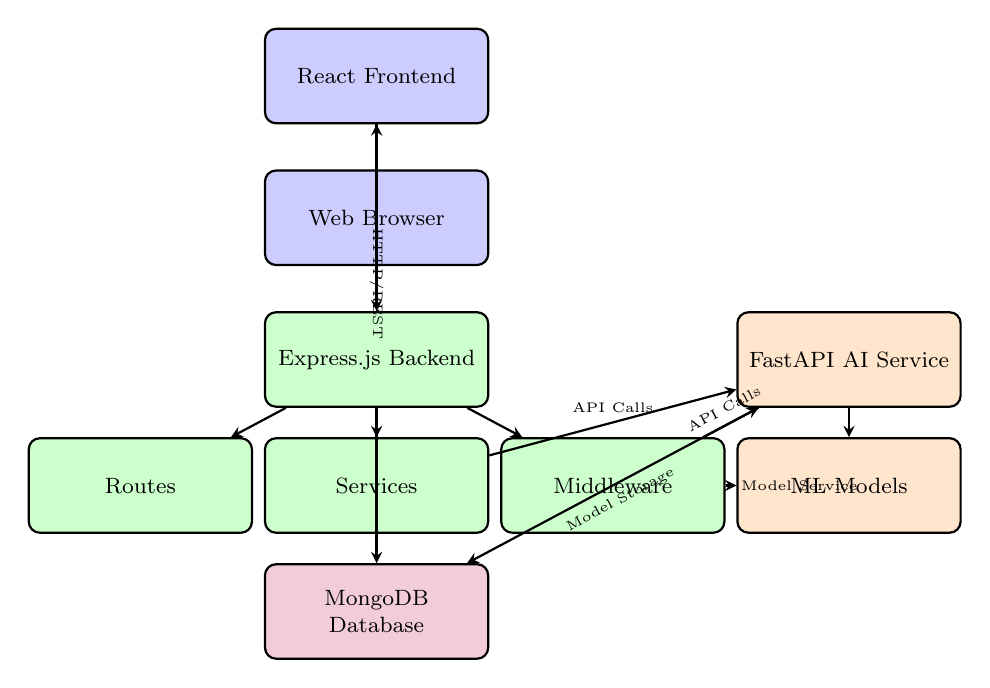
\begin{tikzpicture}[
    box/.style={rectangle, draw=black, thick, minimum width=2.8cm, minimum height=1.2cm, text centered, rounded corners, font=\footnotesize, text width=2.6cm},
    arrow/.style={->, >=stealth, thick, font=\tiny}
]

% Frontend Layer
\node[box, fill=blue!20] (frontend) at (0,6) {React Frontend};
\node[box, fill=blue!20] (browser) at (0,4.2) {Web Browser};

% Backend Layer
\node[box, fill=green!20] (express) at (0,2.4) {Express.js Backend};
\node[box, fill=green!20] (routes) at (-3,0.8) {Routes};
\node[box, fill=green!20] (services) at (0,0.8) {Services};
\node[box, fill=green!20] (middleware) at (3,0.8) {Middleware};

% AI Microservice
\node[box, fill=orange!20] (fastapi) at (6,2.4) {FastAPI AI Service};
\node[box, fill=orange!20] (mlmodels) at (6,0.8) {ML Models};

% Database Layer
\node[box, fill=purple!20] (mongodb) at (0,-0.8) {MongoDB Database};

% Connections
\draw[arrow] (browser) -- (frontend);
\draw[arrow] (frontend) -- node[right, font=\tiny, sloped] {HTTP/REST} (express);
\draw[arrow] (express) -- (routes);
\draw[arrow] (express) -- (services);
\draw[arrow] (express) -- (middleware);
\draw[arrow] (services) -- node[above, font=\tiny] {API Calls} (fastapi);
\draw[arrow] (middleware) -- node[above, font=\tiny, sloped] {API Calls} (fastapi);
\draw[arrow] (middleware) -- node[right, font=\tiny, sloped] {Model Service} (mlmodels);
\draw[arrow] (fastapi) -- (mlmodels);
\draw[arrow] (express) -- (mongodb);
\draw[arrow] (fastapi) -- node[below, sloped, font=\tiny] {Model Storage} (mongodb);

\end{tikzpicture}%
}
\caption{High-Level System Architecture}
\label{fig:architecture}
\end{figure}

\subsection{Architecture Layers}
The system architecture is divided into the following layers:

\begin{enumerate}
    \item \textbf{Presentation Layer}: React frontend for user interface
    \item \textbf{Application Layer}: Express.js backend for business logic and orchestration
    \item \textbf{AI/ML Layer}: Python FastAPI microservice with machine learning models and NLP processors
    \item \textbf{Data Layer}: MongoDB for application data and model storage for AI components
\end{enumerate}

\section{Use Case Diagram}
Figure~\ref{fig:usecase} illustrates the main use cases of the ShifaMart system from a user perspective.

\begin{figure}[H]
\centering
\resizebox{0.95\textwidth}{!}{%
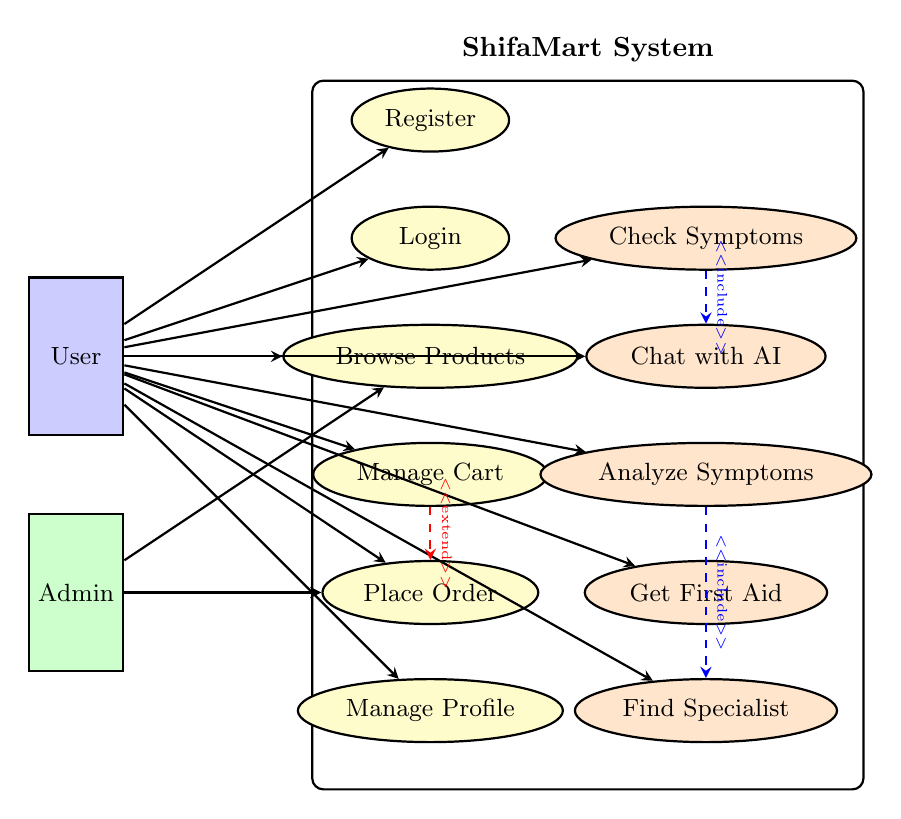
\begin{tikzpicture}[
    usecase/.style={ellipse, draw=black, thick, minimum width=2cm, minimum height=0.8cm, text centered, fill=white, font=\small},
    actorbox/.style={rectangle, draw=black, thick, minimum width=1.2cm, minimum height=2cm, text centered, font=\small},
    arrow/.style={->, >=stealth, thick},
    include/.style={->, >=stealth, dashed, thick, color=blue},
    extend/.style={->, >=stealth, dashed, thick, color=red}
]

% Actors
\node[actorbox, fill=blue!20] (user) at (-3.5,-4) {User};
\node[actorbox, fill=green!20] (admin) at (-3.5,-7) {Admin};

% System boundary
\draw[thick, rounded corners] (-0.5,-0.5) rectangle (6.5,-9.5);

% Use cases - Left column
\node[usecase, fill=yellow!20] (register) at (1,-1) {Register};
\node[usecase, fill=yellow!20] (login) at (1,-2.5) {Login};
\node[usecase, fill=yellow!20] (browse) at (1,-4) {Browse Products};
\node[usecase, fill=yellow!20] (cart) at (1,-5.5) {Manage Cart};
\node[usecase, fill=yellow!20] (order) at (1,-7) {Place Order};
\node[usecase, fill=yellow!20] (profile) at (1,-8.5) {Manage Profile};

% Use cases - Right column (AI features)
\node[usecase, fill=orange!20] (symptom) at (4.5,-2.5) {Check Symptoms};
\node[usecase, fill=orange!20] (chat) at (4.5,-4) {Chat with AI};
\node[usecase, fill=orange!20] (analyze) at (4.5,-5.5) {Analyze Symptoms};
\node[usecase, fill=orange!20] (firstaid) at (4.5,-7) {Get First Aid};
\node[usecase, fill=orange!20] (specialist) at (4.5,-8.5) {Find Specialist};

% Associations from User
\draw[arrow] (user) -- (register);
\draw[arrow] (user) -- (login);
\draw[arrow] (user) -- (browse);
\draw[arrow] (user) -- (cart);
\draw[arrow] (user) -- (order);
\draw[arrow] (user) -- (profile);
\draw[arrow] (user) -- (symptom);
\draw[arrow] (user) -- (chat);
\draw[arrow] (user) -- (analyze);
\draw[arrow] (user) -- (firstaid);
\draw[arrow] (user) -- (specialist);

% Associations from Admin
\draw[arrow] (admin) -- (browse);
\draw[arrow] (admin) -- (order);

% Include relationships
\draw[include] (symptom) -- node[above, sloped, font=\tiny] {<<include>>} (chat);
\draw[include] (analyze) -- node[above, sloped, font=\tiny] {<<include>>} (specialist);

% Extend relationship
\draw[extend] (cart) -- node[above, sloped, font=\tiny] {<<extend>>} (order);

% System label
\node at (3,-0.1) {\textbf{ShifaMart System}};

\end{tikzpicture}%
}
\caption{Use Case Diagram for ShifaMart}
\label{fig:usecase}
\end{figure}

\section{Domain Model}
Figure~\ref{fig:domain} shows the domain model representing the core entities and their relationships in the ShifaMart system.

\begin{figure}[H]
\centering
\resizebox{0.95\textwidth}{!}{%
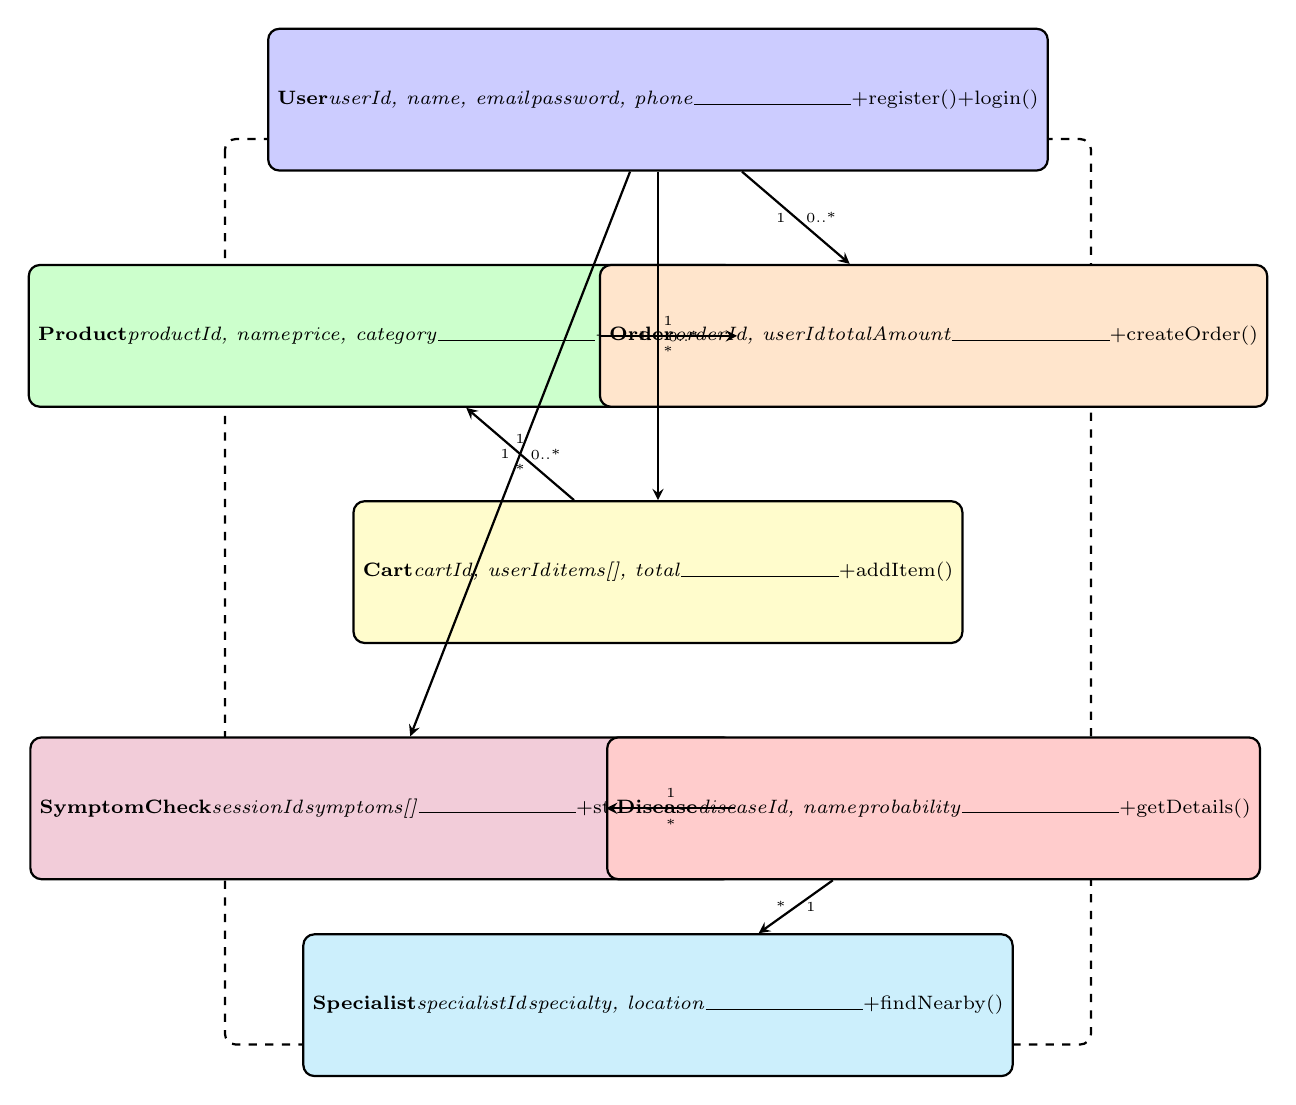
\begin{tikzpicture}[
    class/.style={rectangle, draw=black, thick, minimum width=2.5cm, minimum height=1.8cm, text centered, rounded corners, font=\scriptsize},
    arrow/.style={->, >=stealth, thick},
    label/.style={font=\tiny}
]

% Package boundary
\draw[thick, dashed, rounded corners] (-5.5,-0.5) rectangle (5.5,-12);
\node at (0,-0.1) {\textbf{ShifaMart Domain}};

% Classes
\node[class, fill=blue!20] (user) at (0,0) {
    \textbf{User} \\
    \textit{userId, name, email} \\
    \textit{password, phone} \\
    \rule{2cm}{0.3pt} \\
    +register() \\
    +login()
};

\node[class, fill=green!20] (product) at (-3.5,-3) {
    \textbf{Product} \\
    \textit{productId, name} \\
    \textit{price, category} \\
    \rule{2cm}{0.3pt} \\
    +getDetails()
};

\node[class, fill=orange!20] (order) at (3.5,-3) {
    \textbf{Order} \\
    \textit{orderId, userId} \\
    \textit{totalAmount} \\
    \rule{2cm}{0.3pt} \\
    +createOrder()
};

\node[class, fill=yellow!20] (cart) at (0,-6) {
    \textbf{Cart} \\
    \textit{cartId, userId} \\
    \textit{items[], total} \\
    \rule{2cm}{0.3pt} \\
    +addItem()
};

\node[class, fill=purple!20] (symptom) at (-3.5,-9) {
    \textbf{SymptomCheck} \\
    \textit{sessionId} \\
    \textit{symptoms[]} \\
    \rule{2cm}{0.3pt} \\
    +startSession()
};

\node[class, fill=red!20] (disease) at (3.5,-9) {
    \textbf{Disease} \\
    \textit{diseaseId, name} \\
    \textit{probability} \\
    \rule{2cm}{0.3pt} \\
    +getDetails()
};

\node[class, fill=cyan!20] (specialist) at (0,-11.5) {
    \textbf{Specialist} \\
    \textit{specialistId} \\
    \textit{specialty, location} \\
    \rule{2cm}{0.3pt} \\
    +findNearby()
};

% Relationships
\draw[arrow] (user) -- node[left, label] {1} node[right, label] {0..*} (cart);
\draw[arrow] (user) -- node[left, label] {1} node[right, label] {0..*} (order);
\draw[arrow] (user) -- node[left, label] {1} node[right, label] {0..*} (symptom);
\draw[arrow] (cart) -- node[above, label] {1} node[below, label] {*} (product);
\draw[arrow] (order) -- node[above, label] {1} node[below, label] {*} (product);
\draw[arrow] (symptom) -- node[above, label] {1} node[below, label] {*} (disease);
\draw[arrow] (disease) -- node[right, label] {1} node[left, label] {*} (specialist);

\end{tikzpicture}%
}
\caption{Domain Model for ShifaMart}
\label{fig:domain}
\end{figure}

\section{Frontend Architecture}

\subsection{Overview}
The React frontend is organized into reusable components following modern React patterns. The frontend provides a responsive, user-friendly interface for both e-commerce functionality and AI-powered health assistance.

\subsection{Technology Stack}
The React frontend uses the following technologies:

\begin{table}[H]
\centering
\caption{Frontend Technology Stack}
\label{tab:frontendtech}
\begin{tabularx}{\textwidth}{|l|X|}
\hline
\textbf{Technology} & \textbf{Purpose} \\
\hline
React 18+ & UI framework and component library \\
\hline
React Router & Client-side routing and navigation \\
\hline
Redux Toolkit & State management for global application state \\
\hline
Axios & HTTP client for API communication \\
\hline
Material-UI / Ant Design & UI component library \\
\hline
CSS3 / Styled Components & Styling and theming \\
\hline
React Hook Form & Form handling and validation \\
\hline
\end{tabularx}
\end{table}

\subsection{Component Structure}
Figure~\ref{fig:reactcomponents} shows the React component hierarchy, and Table~\ref{tab:reactcomponents} describes the main React components and their functionality.

\begin{table}[H]
\centering
\caption{React Frontend Components}
\label{tab:reactcomponents}
\begin{tabularx}{\textwidth}{|l|X|}
\hline
\textbf{Component} & \textbf{Description} \\
\hline
App & Main application component, handles routing and global state \\
\hline
Navbar & Navigation bar with menu items, cart icon, user profile \\
\hline
Home & Landing page with featured products and health tips \\
\hline
Products & Product listing page with search, filter, and pagination \\
\hline
ProductDetail & Individual product page with details, reviews, add to cart \\
\hline
Cart & Shopping cart component showing items, quantities, totals \\
\hline
Checkout & Checkout process with address, payment, order summary \\
\hline
Profile & User profile management, order history, settings \\
\hline
SymptomChecker & Main AI health assistant interface \\
\hline
ChatInterface & Chat UI for conversational symptom checking \\
\hline
ResultsDisplay & Displays disease predictions, severity, recommendations \\
\hline
Suggestions & Quick reply buttons for user interaction \\
\hline
FirstAidGuide & Displays first aid instructions for emergencies \\
\hline
SpecialistMap & Shows nearby specialists on map integration \\
\hline
\end{tabularx}
\end{table}

\begin{figure}[H]
\centering
\resizebox{0.85\textwidth}{!}{%
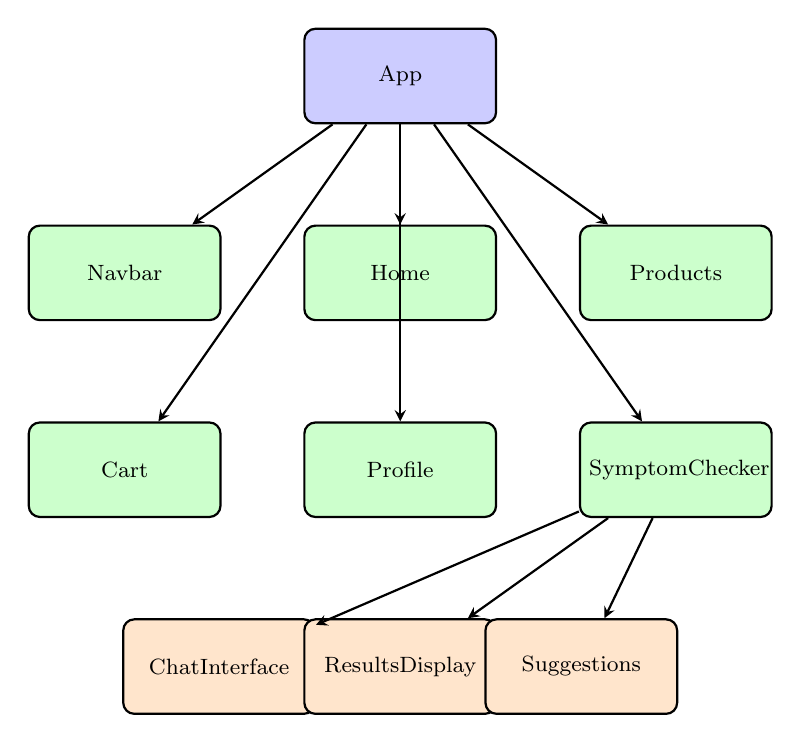
\begin{tikzpicture}[
    component/.style={rectangle, draw=black, thick, minimum width=2.4cm, minimum height=1.2cm, text centered, rounded corners, font=\footnotesize, text width=2.2cm},
    arrow/.style={->, >=stealth, thick}
]

\node[component, fill=blue!20] (app) at (0,0) {App};
\node[component, fill=green!20] (navbar) at (-3.5,-2.5) {Navbar};
\node[component, fill=green!20] (home) at (0,-2.5) {Home};
\node[component, fill=green!20] (products) at (3.5,-2.5) {Products};
\node[component, fill=green!20] (cart) at (-3.5,-5) {Cart};
\node[component, fill=green!20] (profile) at (0,-5) {Profile};
\node[component, fill=green!20] (symptom) at (3.5,-5) {SymptomChecker};
\node[component, fill=orange!20] (chat) at (-2.3,-7.5) {ChatInterface};
\node[component, fill=orange!20] (results) at (0,-7.5) {ResultsDisplay};
\node[component, fill=orange!20] (suggestions) at (2.3,-7.5) {Suggestions};

\draw[arrow] (app) -- (navbar);
\draw[arrow] (app) -- (home);
\draw[arrow] (app) -- (products);
\draw[arrow] (app) -- (cart);
\draw[arrow] (app) -- (profile);
\draw[arrow] (app) -- (symptom);
\draw[arrow] (symptom) -- (chat);
\draw[arrow] (symptom) -- (results);
\draw[arrow] (symptom) -- (suggestions);

\end{tikzpicture}%
}
\caption{React Frontend Component Hierarchy}
\label{fig:reactcomponents}
\end{figure}

\section{Backend Architecture}

\subsection{Overview}
The Express.js backend serves as the main application server, handling:

\begin{itemize}
    \item User authentication and authorization
    \item Product catalog management
    \item Shopping cart and order processing
    \item Payment integration
    \item User profile management
    \item Integration with AI microservice
\end{itemize}

\subsection{API Endpoints}
Table~\ref{tab:backendapi} lists the main backend API endpoints.

\begin{table}[H]
\centering
\caption{Express.js Backend API Endpoints}
\label{tab:backendapi}
\begin{tabularx}{\textwidth}{|l|l|X|}
\hline
\textbf{Method} & \textbf{Endpoint} & \textbf{Description} \\
\hline
POST & /api/auth/register & User registration \\
\hline
POST & /api/auth/login & User authentication \\
\hline
GET & /api/products & Get all products with filters \\
\hline
GET & /api/products/:id & Get product details \\
\hline
POST & /api/cart/add & Add item to cart \\
\hline
GET & /api/cart & Get user's cart \\
\hline
POST & /api/orders & Create new order \\
\hline
GET & /api/orders & Get user's orders \\
\hline
POST & /api/symptom-checker/chat & Chat with AI agent \\
\hline
POST & /api/symptom-checker/analyze & Quick symptom analysis \\
\hline
GET & /api/symptom-checker/symptoms & Get all symptoms list \\
\hline
\end{tabularx}
\end{table}

\subsection{Backend Structure}
The Express.js backend is organized as follows:

\begin{lstlisting}[language=bash, caption=Express.js Backend Structure]
backend/
├── routes/
│   ├── auth.js              # Authentication routes
│   ├── products.js          # Product management
│   ├── orders.js            # Order processing
│   └── symptomChecker.js    # AI service integration
├── services/
│   └── aiService.js         # AI microservice client
├── models/
│   ├── User.js              # User model
│   ├── Product.js           # Product model
│   └── Order.js             # Order model
├── middleware/
│   ├── auth.js              # Authentication middleware
│   └── errorHandler.js      # Error handling
└── app.js                   # Main application file
\end{lstlisting}

\subsection{AI Service Integration}
The Express.js backend integrates with the Python AI microservice through a dedicated service layer:

\begin{lstlisting}[language=JavaScript, caption=AI Service Integration in Express.js]
// backend/services/aiService.js
const axios = require('axios');

const AI_API_URL = process.env.AI_API_URL || 'http://localhost:8000';

class AIService {
  async checkHealth() {
    const response = await axios.get(`${AI_API_URL}/api/health`);
    return response.data;
  }

  async chat(sessionId, message) {
    const response = await axios.post(`${AI_API_URL}/api/chat`, {
      session_id: sessionId,
      message: message
    });
    return response.data;
  }

  async analyze(text) {
    const response = await axios.post(`${AI_API_URL}/api/analyze`, {
      text: text,
      top_k: 5
    });
    return response.data;
  }

  async checkSeverity(symptoms, duration = null) {
    const response = await axios.post(`${AI_API_URL}/api/severity`, {
      symptoms: symptoms,
      duration: duration
    });
    return response.data;
  }
}

module.exports = new AIService();
\end{lstlisting}

\subsection{Express Routes for AI Features}
The backend exposes routes that proxy requests to the AI microservice:

\begin{lstlisting}[language=JavaScript, caption=Express Routes for Symptom Checker]
// backend/routes/symptomChecker.js
const express = require('express');
const router = express.Router();
const aiService = require('../services/aiService');

router.post('/chat', async (req, res) => {
  try {
    const { sessionId, message } = req.body;
    const session = sessionId || `${req.user?._id || 'guest'}_${Date.now()}`;
    const response = await aiService.chat(session, message);
    
    if (response.is_emergency) {
      // Log emergency for monitoring
      console.log(`⚠️ EMERGENCY detected for session: ${session}`);
    }
    
    res.json({ ...response, sessionId: session });
  } catch (error) {
    res.status(500).json({ error: 'AI chat error', details: error.message });
  }
});

router.post('/analyze', async (req, res) => {
  try {
    const { text } = req.body;
    const response = await aiService.analyze(text);
    res.json(response);
  } catch (error) {
    res.status(500).json({ error: 'Analysis error', details: error.message });
  }
});
\end{lstlisting}

\section{AI Microservice Architecture}

\subsection{Overview}
The Python-based AI microservice is built using FastAPI and provides all AI-related functionality as a separate, scalable service.

\subsection{Microservice Components}
The AI microservice consists of:

\begin{itemize}
    \item \textbf{Disease Prediction Model}: Ensemble of XGBoost and Random Forest classifiers
    \item \textbf{NLP Processor}: Natural language understanding for symptom extraction
    \item \textbf{Severity Detection Model}: Gradient Boosting classifier for severity assessment
    \item \textbf{First Aid System}: Rule-based first-aid guidance system
    \item \textbf{Conversational Agent}: State machine-based chat interface
    \item \textbf{Specialist Mapper}: Disease-to-specialist recommendation system
    \item \textbf{Maps Integration}: Location-based doctor search
    \item \textbf{API Server}: FastAPI-based RESTful API
\end{itemize}

\subsection{FastAPI Application Structure}
\begin{lstlisting}[language=Python, caption=FastAPI Application Structure]
# mern_api.py - Main FastAPI application
from fastapi import FastAPI, HTTPException
from fastapi.middleware.cors import CORSMiddleware
from contextlib import asynccontextmanager

# Import AI components
from disease_predictor import DiseasePredictionModel
from symptom_checker_v2 import EnhancedSymptomChecker
from nlp_processor import SymptomNLPProcessor
from severity_model import SeverityDetectionModel
from first_aid import FirstAidSystem

# Global AI components
disease_model = None
symptom_agent = None
nlp_processor = None
severity_model = None
first_aid_system = None

@asynccontextmanager
async def lifespan(app: FastAPI):
    """Initialize AI models on startup"""
    global disease_model, symptom_agent, nlp_processor, severity_model, first_aid_system
    
    # Initialize components
    disease_model = DiseasePredictionModel()
    symptom_agent = EnhancedSymptomChecker(disease_model)
    nlp_processor = SymptomNLPProcessor()
    severity_model = SeverityDetectionModel()
    first_aid_system = FirstAidSystem()
    
    # Load all models
    symptom_agent.load_all_models()
    nlp_processor.set_known_symptoms(disease_model.get_all_symptoms())
    
    yield  # App runs here
    
    # Cleanup (if needed)

app = FastAPI(
    title="ShifaMart+ AI API (MERN Integration)",
    version="2.0.0",
    lifespan=lifespan
)

# CORS Configuration for MERN integration
app.add_middleware(
    CORSMiddleware,
    allow_origins=["*"],  # Configure for production
    allow_credentials=True,
    allow_methods=["*"],
    allow_headers=["*"],
)
\end{lstlisting}

\subsection{API Endpoints}
The AI microservice exposes the following endpoints:

\begin{itemize}
    \item \texttt{POST /api/chat}: Conversational AI for symptom checking
    \item \texttt{POST /api/analyze}: Quick text-based symptom analysis
    \item \texttt{POST /api/predict}: Direct prediction from symptom list
    \item \texttt{POST /api/severity}: Severity assessment
    \item \texttt{POST /api/first-aid}: First aid guidance
    \item \texttt{GET /api/symptoms}: List all known symptoms
    \item \texttt{GET /api/diseases}: List all known diseases
    \item \texttt{GET /api/health}: Health check endpoint
\end{itemize}

\section{Database Design}

\subsection{Database Schema}
Figure~\ref{fig:database} shows the MongoDB database schema with collections and their relationships.

\begin{figure}[H]
\centering
\resizebox{0.9\textwidth}{!}{%
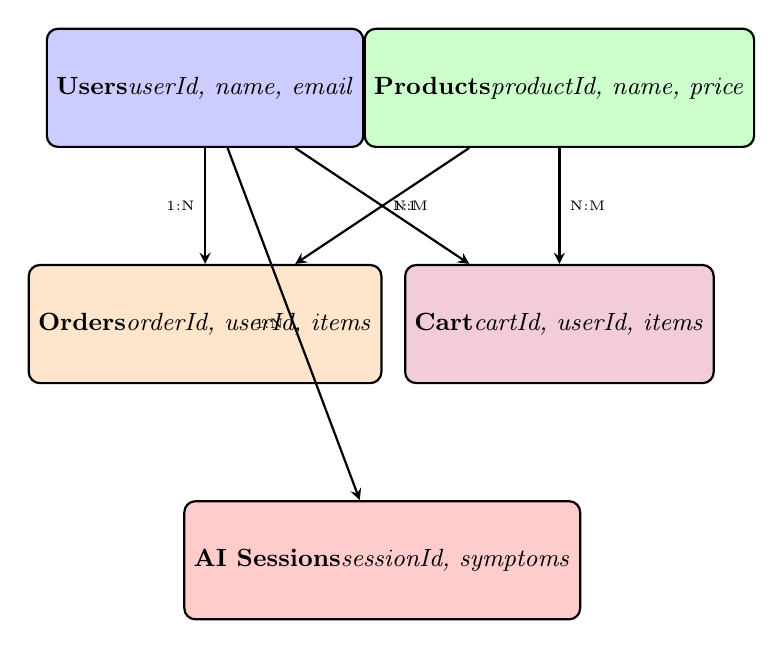
\begin{tikzpicture}[
    collection/.style={rectangle, draw=black, thick, minimum width=2.5cm, minimum height=1.5cm, text centered, rounded corners, font=\small},
    arrow/.style={->, >=stealth, thick}
]

\node[collection, fill=blue!20] (users) at (0,0) {
    \textbf{Users} \\
    \textit{userId, name, email}
};

\node[collection, fill=green!20] (products) at (4.5,0) {
    \textbf{Products} \\
    \textit{productId, name, price}
};

\node[collection, fill=orange!20] (orders) at (0,-3) {
    \textbf{Orders} \\
    \textit{orderId, userId, items}
};

\node[collection, fill=purple!20] (cart) at (4.5,-3) {
    \textbf{Cart} \\
    \textit{cartId, userId, items}
};

\node[collection, fill=red!20] (sessions) at (2.25,-6) {
    \textbf{AI Sessions} \\
    \textit{sessionId, symptoms}
};

\draw[arrow] (users) -- node[left, font=\tiny] {1:N} (orders);
\draw[arrow] (users) -- node[right, font=\tiny] {1:1} (cart);
\draw[arrow] (users) -- node[left, font=\tiny] {1:N} (sessions);
\draw[arrow] (products) -- node[right, font=\tiny] {N:M} (orders);
\draw[arrow] (products) -- node[right, font=\tiny] {N:M} (cart);

\end{tikzpicture}%
}
\caption{MongoDB Database Schema}
\label{fig:database}
\end{figure}

\section{AI Model Development}

\subsection{Data Preprocessing}
The data preprocessing module handles loading and transformation of medical datasets.

\subsubsection{Dataset Structure}
The system uses four main datasets:

\begin{enumerate}
    \item \textbf{Main Dataset} (\texttt{dataset.csv}): Contains 4,922 symptom-disease mappings
    \item \textbf{Symptom Description} (\texttt{symptom\_Description.csv}): Disease descriptions
    \item \textbf{Symptom Precaution} (\texttt{symptom\_precaution.csv}): Precautions for each disease
    \item \textbf{Symptom Severity} (\texttt{Symptom-severity.csv}): Severity weights for symptoms
\end{enumerate}

\subsubsection{Dataset Statistics}
Table~\ref{tab:dataset} provides detailed statistics about the datasets used.

\begin{table}[H]
\centering
\caption{Dataset Statistics}
\label{tab:dataset}
\begin{tabularx}{0.6\textwidth}{|l|X|}
\hline
\textbf{Statistic} & \textbf{Value} \\
\hline
Total Records & 4,922 \\
\hline
Number of Diseases & 41 \\
\hline
Number of Symptoms & 132 \\
\hline
Average Symptoms per Disease & 5-8 \\
\hline
Most Common Disease & Common Cold \\
\hline
Dataset Format & CSV \\
\hline
Training Set Size & 3,937 (80\%) \\
\hline
Test Set Size & 985 (20\%) \\
\hline
\end{tabularx}
\end{table}

\subsection{Disease Prediction Model}
The disease prediction model uses an ensemble approach combining XGBoost and Random Forest classifiers.

\subsubsection{Model Architecture}
The ensemble model consists of:

\begin{itemize}
    \item \textbf{Random Forest Classifier}: 100 estimators, max depth 15, balanced class weights
    \item \textbf{XGBoost Classifier}: 100 estimators, max depth 6, learning rate 0.1
    \item \textbf{Voting Classifier}: Soft voting using probability distributions
\end{itemize}

\subsubsection{Model Hyperparameters}
Table~\ref{tab:hyperparameters} shows the hyperparameters used for each model.

\begin{table}[H]
\centering
\caption{Model Hyperparameters}
\label{tab:hyperparameters}
\begin{tabularx}{0.8\textwidth}{|l|X|X|}
\hline
\textbf{Parameter} & \textbf{Random Forest} & \textbf{XGBoost} \\
\hline
n\_estimators & 100 & 100 \\
\hline
max\_depth & 15 & 6 \\
\hline
learning\_rate & N/A & 0.1 \\
\hline
min\_samples\_split & 5 & N/A \\
\hline
min\_samples\_leaf & 2 & N/A \\
\hline
class\_weight & balanced & N/A \\
\hline
subsample & N/A & 0.8 \\
\hline
colsample\_bytree & N/A & 0.8 \\
\hline
random\_state & 42 & 42 \\
\hline
\end{tabularx}
\end{table}

\subsection{Natural Language Processing}
The NLP processor extracts symptoms from natural language descriptions using synonym mapping, pattern matching, and fuzzy matching techniques.

\subsubsection{NLP Processing Pipeline}
Table~\ref{tab:nlppipeline} describes the NLP processing steps.

\begin{table}[H]
\centering
\caption{NLP Processing Pipeline}
\label{tab:nlppipeline}
\begin{tabularx}{\textwidth}{|c|X|}
\hline
\textbf{Step} & \textbf{Description} \\
\hline
1 & Text preprocessing: lowercase, contraction expansion, punctuation normalization \\
\hline
2 & Synonym matching: Match user text against 132+ symptom synonyms \\
\hline
3 & Direct matching: Match against known symptom names \\
\hline
4 & Fuzzy matching: Match common symptom words \\
\hline
5 & Negation detection: Identify negated symptoms \\
\hline
6 & Duration extraction: Extract temporal information (days, weeks, hours) \\
\hline
7 & Severity modifier detection: Identify severity indicators (mild, severe, etc.) \\
\hline
8 & Confidence scoring: Assign confidence scores to extracted symptoms \\
\hline
\end{tabularx}
\end{table}

\subsection{Severity Detection Model}
The severity detection model classifies symptoms into four levels: MILD, MODERATE, SEVERE, and EMERGENCY, using a hybrid rule-based and ML approach.

\subsubsection{Severity Classification}
Table~\ref{tab:severity} shows the severity levels and their characteristics.

\begin{table}[H]
\centering
\caption{Severity Level Classification}
\label{tab:severity}
\begin{tabularx}{\textwidth}{|l|X|X|}
\hline
\textbf{Level} & \textbf{Score Range} & \textbf{Description} \\
\hline
MILD & 0.0 - 3.0 & Low-risk symptoms requiring home care and rest \\
\hline
MODERATE & 3.0 - 5.0 & Symptoms that should be monitored; consider doctor visit \\
\hline
SEVERE & 5.0 - 7.0 & Serious symptoms requiring medical attention soon \\
\hline
EMERGENCY & 7.0+ & Critical symptoms requiring immediate medical care \\
\hline
\end{tabularx}
\end{table}

\subsection{First Aid System}
The first aid system provides step-by-step guidance for 12+ emergency types including heart attack, stroke, breathing difficulty, and more.

\subsection{Conversational AI Agent}
The conversational agent uses a state machine with states: GREETING, COLLECTING\_SYMPTOMS, ASKING\_DURATION, CONFIRMING\_SYMPTOMS, SHOWING\_RESULTS, EMERGENCY\_DETECTED, and ASKING\_CITY.

\subsubsection{State Transition Diagram}
Figure~\ref{fig:statetransition} shows the state transition diagram for the conversational AI agent.

\begin{figure}[H]
\centering
\resizebox{0.95\textwidth}{!}{%
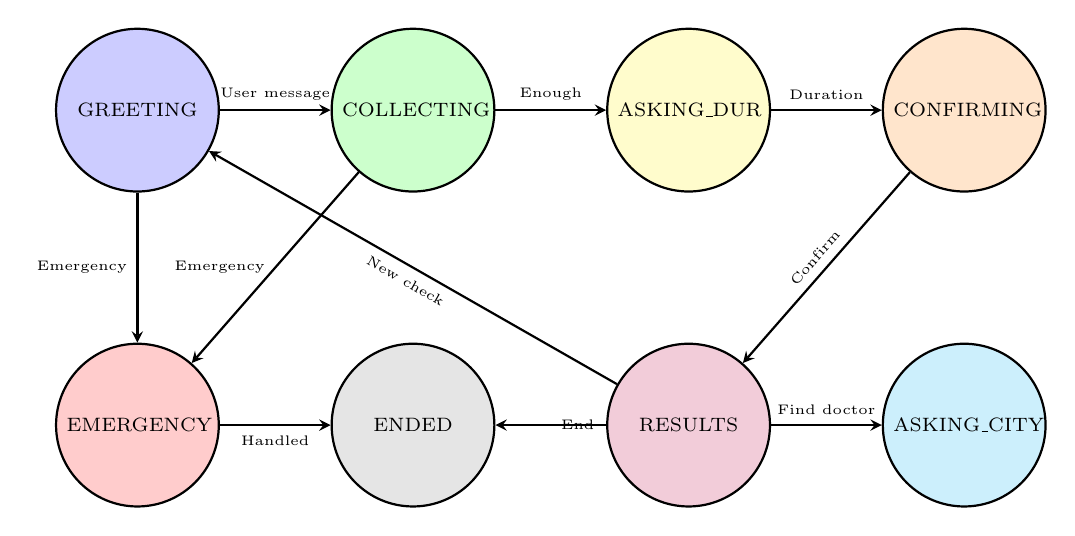
\begin{tikzpicture}[
    state/.style={circle, draw=black, thick, minimum size=2cm, text centered, font=\scriptsize, text width=1.8cm},
    arrow/.style={->, >=stealth, thick, font=\tiny}
]

\node[state, fill=blue!20] (greeting) at (0,0) {GREETING};
\node[state, fill=green!20] (collecting) at (3.5,0) {COLLECTING};
\node[state, fill=yellow!20] (duration) at (7,0) {ASKING\_DUR};
\node[state, fill=orange!20] (confirming) at (10.5,0) {CONFIRMING};
\node[state, fill=purple!20] (results) at (7,-4) {RESULTS};
\node[state, fill=red!20] (emergency) at (0,-4) {EMERGENCY};
\node[state, fill=cyan!20] (city) at (10.5,-4) {ASKING\_CITY};
\node[state, fill=gray!20] (ended) at (3.5,-4) {ENDED};

\draw[arrow] (greeting) -- node[above, font=\tiny, sloped] {User message} (collecting);
\draw[arrow] (greeting) -- node[left, font=\tiny] {Emergency} (emergency);
\draw[arrow] (collecting) -- node[above, font=\tiny] {Enough} (duration);
\draw[arrow] (duration) -- node[above, font=\tiny] {Duration} (confirming);
\draw[arrow] (confirming) -- node[above, font=\tiny, sloped] {Confirm} (results);
\draw[arrow] (collecting) -- node[left, font=\tiny] {Emergency} (emergency);
\draw[arrow] (results) -- node[above, font=\tiny] {Find doctor} (city);
\draw[arrow] (results) -- node[below, font=\tiny, sloped] {New check} (greeting);
\draw[arrow] (results) -- node[right, font=\tiny] {End} (ended);
\draw[arrow] (emergency) -- node[below, font=\tiny] {Handled} (ended);

\end{tikzpicture}%
}
\caption{State Transition Diagram for Conversational AI Agent}
\label{fig:statetransition}
\end{figure}

\section{System Integration}

\subsection{Integration Flow}
The complete integration flow works as follows:

\begin{enumerate}
    \item User interacts with React frontend
    \item Frontend sends requests to Express.js backend
    \item Express.js backend routes AI-related requests to AI service
    \item AI service processes request using ML models
    \item Response is returned through Express.js to frontend
    \item Frontend displays results to user
\end{enumerate}

\subsection{Sequence Diagrams}

\subsubsection{Symptom Checking Flow}
Figure~\ref{fig:sequence} shows the sequence diagram for the symptom checking process.

\begin{figure}[H]
\centering
\resizebox{0.9\textwidth}{!}{%
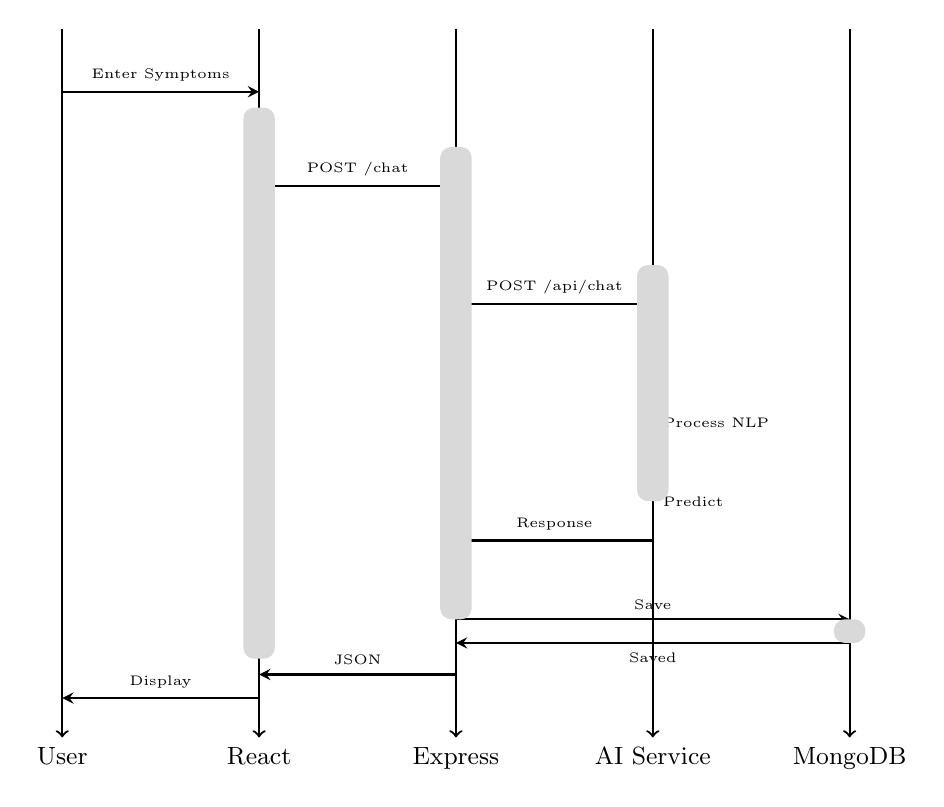
\begin{tikzpicture}[
    lifeline/.style={draw=black, thick, ->},
    activation/.style={fill=gray!30, rectangle, rounded corners},
    message/.style={->, >=stealth, thick, font=\tiny}
]

% Lifelines
\draw[lifeline] (0,0) -- (0,-9) node[below, font=\small] {User};
\draw[lifeline] (2.5,0) -- (2.5,-9) node[below, font=\small] {React};
\draw[lifeline] (5,0) -- (5,-9) node[below, font=\small] {Express};
\draw[lifeline] (7.5,0) -- (7.5,-9) node[below, font=\small] {AI Service};
\draw[lifeline] (10,0) -- (10,-9) node[below, font=\small] {MongoDB};

% Messages
\draw[message] (0,-0.8) -- (2.5,-0.8) node[midway, above, font=\tiny] {Enter Symptoms};
\draw[message] (2.5,-2) -- (5,-2) node[midway, above, font=\tiny] {POST /chat};
\draw[message] (5,-3.5) -- (7.5,-3.5) node[midway, above, font=\tiny] {POST /api/chat};
\draw[message] (7.5,-4.5) -- (7.5,-5) node[right, font=\tiny] {Process NLP};
\draw[message] (7.5,-5.5) -- (7.5,-6) node[right, font=\tiny] {Predict};
\draw[message] (7.5,-6.5) -- (5,-6.5) node[midway, above, font=\tiny] {Response};
\draw[message] (5,-7.5) -- (10,-7.5) node[midway, above, font=\tiny] {Save};
\draw[message] (10,-7.8) -- (5,-7.8) node[midway, below, font=\tiny] {Saved};
\draw[message] (5,-8.2) -- (2.5,-8.2) node[midway, above, font=\tiny] {JSON};
\draw[message] (2.5,-8.5) -- (0,-8.5) node[midway, above, font=\tiny] {Display};

% Activations
\fill[activation] (2.3,-1) rectangle (2.7,-8);
\fill[activation] (4.8,-1.5) rectangle (5.2,-7.5);
\fill[activation] (7.3,-3) rectangle (7.7,-6);
\fill[activation] (9.8,-7.5) rectangle (10.2,-7.8);

\end{tikzpicture}%
}
\caption{Sequence Diagram for Symptom Checking}
\label{fig:sequence}
\end{figure}

\subsubsection{Order Placement Flow}
Figure~\ref{fig:ssd} shows the system sequence diagram for placing an order.

\begin{figure}[H]
\centering
\resizebox{0.8\textwidth}{!}{%
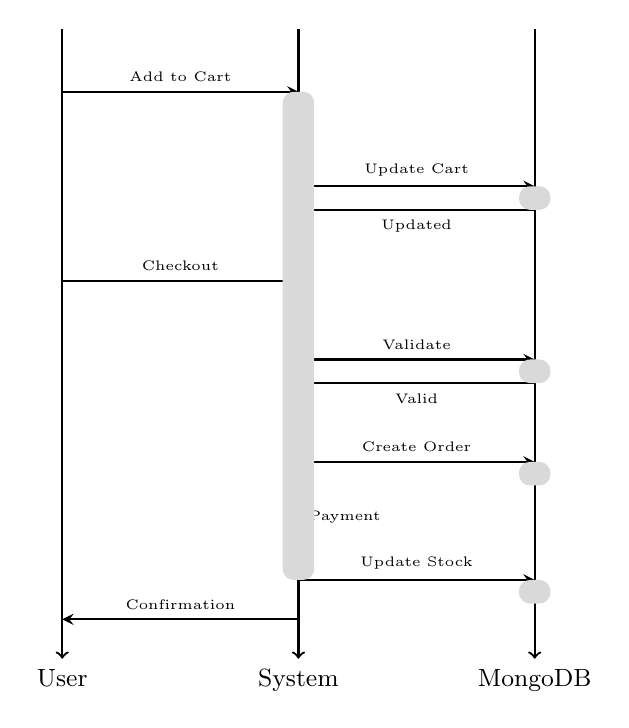
\begin{tikzpicture}[
    lifeline/.style={draw=black, thick, ->},
    activation/.style={fill=gray!30, rectangle, rounded corners},
    message/.style={->, >=stealth, thick, font=\tiny}
]

% Lifelines
\draw[lifeline] (0,0) -- (0,-8) node[below, font=\small] {User};
\draw[lifeline] (3,0) -- (3,-8) node[below, font=\small] {System};
\draw[lifeline] (6,0) -- (6,-8) node[below, font=\small] {MongoDB};

% Messages
\draw[message] (0,-0.8) -- (3,-0.8) node[midway, above, font=\tiny] {Add to Cart};
\draw[message] (3,-2) -- (6,-2) node[midway, above, font=\tiny] {Update Cart};
\draw[message] (6,-2.3) -- (3,-2.3) node[midway, below, font=\tiny] {Updated};
\draw[message] (0,-3.2) -- (3,-3.2) node[midway, above, font=\tiny] {Checkout};
\draw[message] (3,-4.2) -- (6,-4.2) node[midway, above, font=\tiny] {Validate};
\draw[message] (6,-4.5) -- (3,-4.5) node[midway, below, font=\tiny] {Valid};
\draw[message] (3,-5.5) -- (6,-5.5) node[midway, above, font=\tiny] {Create Order};
\draw[message] (3,-6.2) -- (3,-6.2) node[right, font=\tiny] {Payment};
\draw[message] (3,-7) -- (6,-7) node[midway, above, font=\tiny] {Update Stock};
\draw[message] (3,-7.5) -- (0,-7.5) node[midway, above, font=\tiny] {Confirmation};

% Activations
\fill[activation] (2.8,-0.8) rectangle (3.2,-7);
\fill[activation] (5.8,-2) rectangle (6.2,-2.3);
\fill[activation] (5.8,-4.2) rectangle (6.2,-4.5);
\fill[activation] (5.8,-5.5) rectangle (6.2,-5.8);
\fill[activation] (5.8,-7) rectangle (6.2,-7.3);

\end{tikzpicture}%
}
\caption{System Sequence Diagram for Order Placement}
\label{fig:ssd}
\end{figure}

\section{System Diagrams}

\subsection{Class Diagram}
Figure~\ref{fig:class} shows the class diagram for the main components of the ShifaMart system.

\begin{figure}[H]
\centering
\resizebox{0.95\textwidth}{!}{%
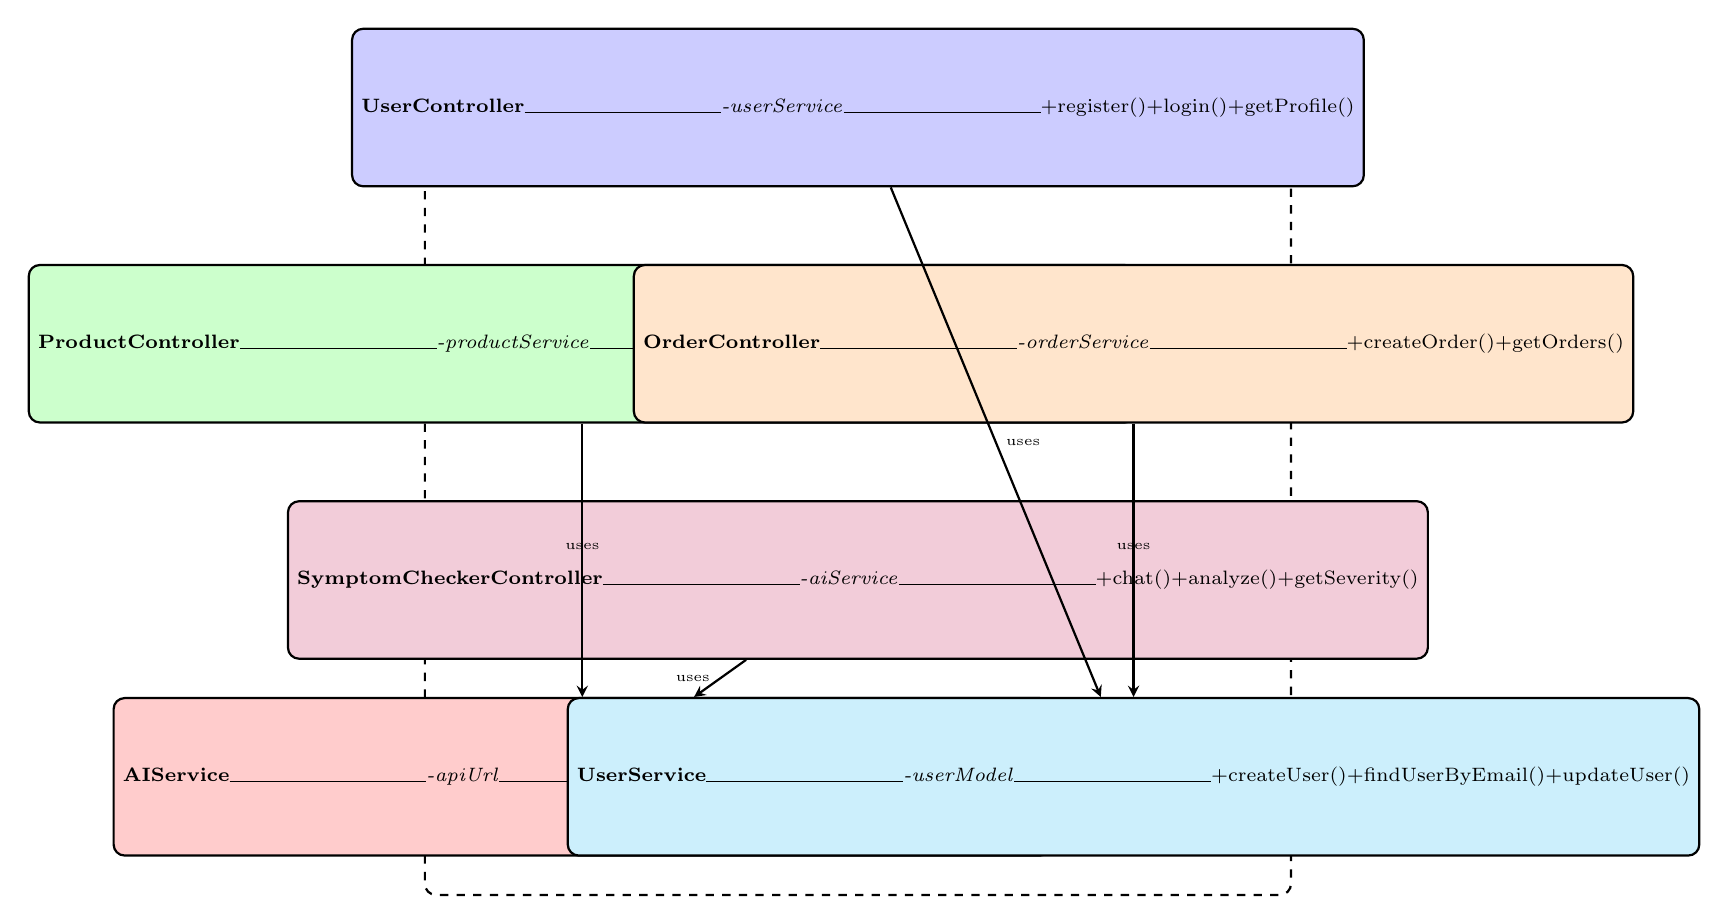
\begin{tikzpicture}[
    class/.style={rectangle, draw=black, thick, minimum width=2.8cm, minimum height=2cm, text centered, rounded corners, font=\scriptsize},
    arrow/.style={->, >=stealth, thick},
    label/.style={font=\tiny}
]

% Package boundary
\draw[thick, dashed, rounded corners] (-5.5,-0.5) rectangle (5.5,-10);
\node at (0,-0.1) {\textbf{Backend Classes}};

% Controller classes
\node[class, fill=blue!20] (userctrl) at (0,0) {
    \textbf{UserController} \\
    \rule{2.5cm}{0.3pt} \\
    \textit{-userService} \\
    \rule{2.5cm}{0.3pt} \\
    +register() \\
    +login() \\
    +getProfile()
};

\node[class, fill=green!20] (productctrl) at (-3.5,-3) {
    \textbf{ProductController} \\
    \rule{2.5cm}{0.3pt} \\
    \textit{-productService} \\
    \rule{2.5cm}{0.3pt} \\
    +getProducts() \\
    +getProductById()
};

\node[class, fill=orange!20] (orderctrl) at (3.5,-3) {
    \textbf{OrderController} \\
    \rule{2.5cm}{0.3pt} \\
    \textit{-orderService} \\
    \rule{2.5cm}{0.3pt} \\
    +createOrder() \\
    +getOrders()
};

\node[class, fill=purple!20] (symptomctrl) at (0,-6) {
    \textbf{SymptomCheckerController} \\
    \rule{2.5cm}{0.3pt} \\
    \textit{-aiService} \\
    \rule{2.5cm}{0.3pt} \\
    +chat() \\
    +analyze() \\
    +getSeverity()
};

% Service classes
\node[class, fill=red!20] (aiservice) at (-3.5,-8.5) {
    \textbf{AIService} \\
    \rule{2.5cm}{0.3pt} \\
    \textit{-apiUrl} \\
    \rule{2.5cm}{0.3pt} \\
    +chat() \\
    +analyze() \\
    +checkSeverity()
};

\node[class, fill=cyan!20] (userservice) at (3.5,-8.5) {
    \textbf{UserService} \\
    \rule{2.5cm}{0.3pt} \\
    \textit{-userModel} \\
    \rule{2.5cm}{0.3pt} \\
    +createUser() \\
    +findUserByEmail() \\
    +updateUser()
};

% Relationships
\draw[arrow] (symptomctrl) -- node[left, label] {uses} (aiservice);
\draw[arrow] (userctrl) -- node[right, label] {uses} (userservice);
\draw[arrow] (productctrl) -- node[above, label] {uses} (aiservice);
\draw[arrow] (orderctrl) -- node[above, label] {uses} (userservice);

\end{tikzpicture}%
}
\caption{Class Diagram for Backend Controllers and Services}
\label{fig:class}
\end{figure}

\subsection{Activity Diagram}
Figure~\ref{fig:activity} shows the activity diagram for the complete symptom checking workflow.

\begin{figure}[H]
\centering
\resizebox{0.9\textwidth}{!}{%
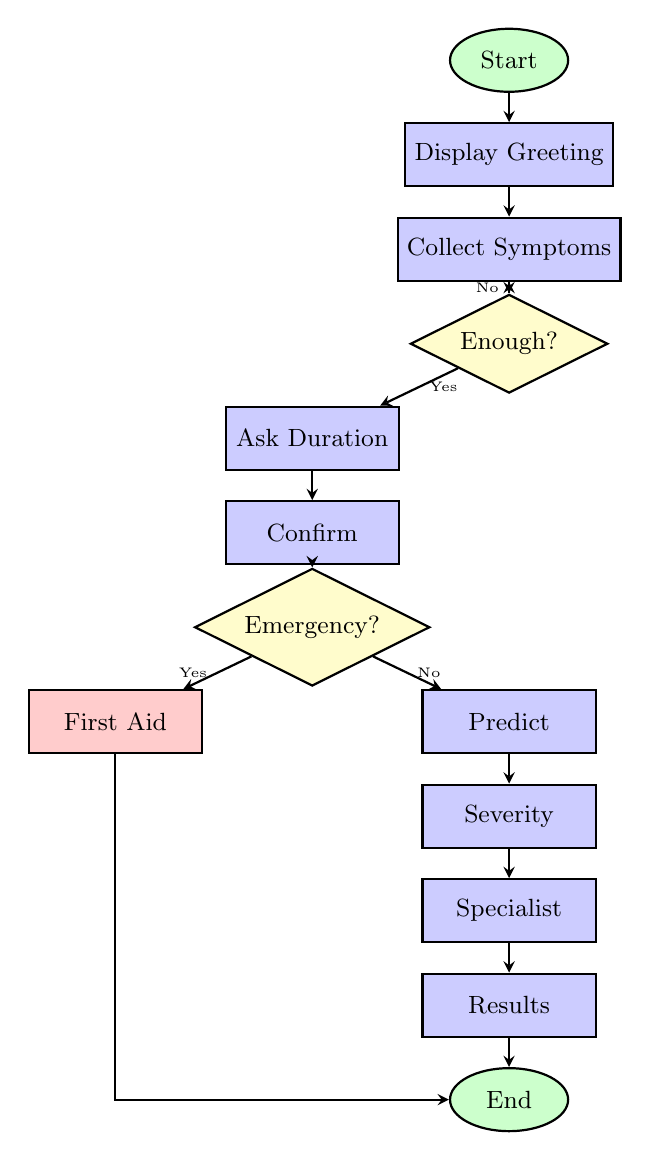
\begin{tikzpicture}[
    node distance=1.2cm,
    startstop/.style={ellipse, draw=black, thick, minimum width=1.5cm, minimum height=0.8cm, text centered, font=\small},
    process/.style={rectangle, draw=black, thick, minimum width=2.2cm, minimum height=0.8cm, text centered, font=\small},
    decision/.style={diamond, draw=black, thick, minimum width=1.5cm, minimum height=0.8cm, text centered, aspect=2, font=\small},
    arrow/.style={->, >=stealth, thick}
]

\node[startstop, fill=green!20] (start) {Start};
\node[process, fill=blue!20, below of=start] (greet) {Display Greeting};
\node[process, fill=blue!20, below of=greet] (collect) {Collect Symptoms};
\node[decision, fill=yellow!20, below of=collect] (enough) {Enough?};
\node[process, fill=blue!20, below of=enough, xshift=-2.5cm] (askduration) {Ask Duration};
\node[process, fill=blue!20, below of=askduration] (confirm) {Confirm};
\node[decision, fill=yellow!20, below of=confirm] (emergency) {Emergency?};
\node[process, fill=red!20, below of=emergency, xshift=-2.5cm] (firstaid) {First Aid};
\node[process, fill=blue!20, below of=emergency, xshift=2.5cm] (predict) {Predict};
\node[process, fill=blue!20, below of=predict] (severity) {Severity};
\node[process, fill=blue!20, below of=severity] (specialist) {Specialist};
\node[process, fill=blue!20, below of=specialist] (results) {Results};
\node[startstop, fill=green!20, below of=results] (end) {End};

\draw[arrow] (start) -- (greet);
\draw[arrow] (greet) -- (collect);
\draw[arrow] (collect) -- (enough);
\draw[arrow] (enough) -- node[left, font=\tiny] {No} (collect);
\draw[arrow] (enough) -- node[right, font=\tiny] {Yes} (askduration);
\draw[arrow] (askduration) -- (confirm);
\draw[arrow] (confirm) -- (emergency);
\draw[arrow] (emergency) -- node[left, font=\tiny] {Yes} (firstaid);
\draw[arrow] (emergency) -- node[right, font=\tiny] {No} (predict);
\draw[arrow] (firstaid) |- (end);
\draw[arrow] (predict) -- (severity);
\draw[arrow] (severity) -- (specialist);
\draw[arrow] (specialist) -- (results);
\draw[arrow] (results) -- (end);

\end{tikzpicture}%
}
\caption{Activity Diagram for Symptom Checking Workflow}
\label{fig:activity}
\end{figure}

\subsection{Event Response Table}
Table~\ref{tab:events} shows the event response table for the conversational AI agent.

\begin{table}[H]
\centering
\caption{Event Response Table for Conversational AI Agent}
\label{tab:events}
\small
\begin{tabularx}{\textwidth}{|X|X|X|X|X|}
\hline
\textbf{Event} & \textbf{Current State} & \textbf{Condition} & \textbf{Action} & \textbf{Next State} \\
\hline
User message & GREETING & Message length $>$ 2 & Extract symptoms, Start collection & COLLECTING\_SYMPTOMS \\
\hline
User message & COLLECTING\_SYMPTOMS & "done" or "analyze" & Ask duration & ASKING\_DURATION \\
\hline
User message & COLLECTING\_SYMPTOMS & Emergency symptoms detected & Show first aid, Alert & EMERGENCY\_DETECTED \\
\hline
User message & ASKING\_DURATION & Duration provided & Confirm symptoms & CONFIRMING\_SYMPTOMS \\
\hline
User message & ASKING\_DURATION & Duration not provided & Ask again or skip & ASKING\_DURATION \\
\hline
User message & CONFIRMING\_SYMPTOMS & "yes" or "analyze" & Run predictions & SHOWING\_RESULTS \\
\hline
User message & SHOWING\_RESULTS & "find doctor" & Ask for city & ASKING\_CITY \\
\hline
User message & SHOWING\_RESULTS & "new" or "start over" & Reset session & GREETING \\
\hline
User message & EMERGENCY\_DETECTED & Any message & Show emergency info & EMERGENCY\_DETECTED \\
\hline
User message & ASKING\_CITY & City name provided & Find specialists & SHOWING\_RESULTS \\
\hline
Session timeout & Any state & 30 min inactivity & End session & ENDED \\
\hline
\end{tabularx}
\end{table}

\section{Implementation Summary}

\subsection{Technology Stack}
The system is implemented using:

\begin{itemize}
    \item \textbf{Frontend}: React.js, HTML5, CSS3, JavaScript
    \item \textbf{Backend}: Node.js, Express.js, MongoDB
    \item \textbf{AI Microservice}: Python 3.8+, FastAPI, scikit-learn, XGBoost
    \item \textbf{Communication}: RESTful APIs, HTTP/JSON
    \item \textbf{Deployment}: Docker (optional), cloud platforms
\end{itemize}

\subsection{Diagram Overview}
Table~\ref{tab:diagrams} provides an overview of all diagrams included in this chapter.

\begin{table}[H]
\centering
\caption{Overview of System Diagrams}
\label{tab:diagrams}
\begin{tabularx}{\textwidth}{|X|X|X|}
\hline
\textbf{Diagram Type} & \textbf{Figure Reference} & \textbf{Description} \\
\hline
High-Level Architecture & Figure~\ref{fig:architecture} & Shows overall system components and connections \\
\hline
Use Case Diagram & Figure~\ref{fig:usecase} & Illustrates user interactions with the system \\
\hline
Domain Model & Figure~\ref{fig:domain} & Represents core entities and relationships \\
\hline
React Components & Figure~\ref{fig:reactcomponents} & Frontend component hierarchy \\
\hline
Database Schema & Figure~\ref{fig:database} & MongoDB collections and relationships \\
\hline
State Transition & Figure~\ref{fig:statetransition} & AI agent state machine \\
\hline
Sequence Diagram & Figure~\ref{fig:sequence} & Symptom checking interaction flow \\
\hline
System Sequence & Figure~\ref{fig:ssd} & Order placement system flow \\
\hline
Class Diagram & Figure~\ref{fig:class} & Backend classes and relationships \\
\hline
Activity Diagram & Figure~\ref{fig:activity} & Symptom checking workflow \\
\hline
Deployment Diagram & Figure~\ref{fig:deployment} & Production deployment architecture \\
\hline
Data Flow Diagram & Figure~\ref{fig:dataflow} & Data flow for symptom checking \\
\hline
Component Interaction & Figure~\ref{fig:component} & Component interactions in MERN stack \\
\hline
Event Response Table & Table~\ref{tab:events} & AI agent event handling \\
\hline
\end{tabularx}
\end{table}

% ============================================================================
% CHAPTER 4: RESULTS AND DISCUSSION
% ============================================================================

\chapter{Results and Discussion}
\vspace{0.5cm}

\section{Introduction}
This chapter presents the experimental results, performance evaluation, and discussion of the ShifaMart platform, with focus on the AI-powered symptom checker feature. The evaluation covers model accuracy, system performance, user experience, and limitations.

\section{Model Performance}
\subsection{Disease Prediction Accuracy}
The ensemble model (XGBoost + Random Forest) achieved the following performance:

\begin{table}[H]
\centering
\caption{Model Performance Metrics}
\label{tab:modelperformance}
\begin{tabularx}{0.7\textwidth}{|l|X|}
\hline
\textbf{Metric} & \textbf{Value} \\
\hline
Overall Accuracy & 92-96\% \\
\hline
Random Forest Accuracy & 91-94\% \\
\hline
XGBoost Accuracy & 93-95\% \\
\hline
Ensemble Accuracy & 92-96\% \\
\hline
Average Precision & 0.89 \\
\hline
Average Recall & 0.87 \\
\hline
Average F1-Score & 0.88 \\
\hline
Training Time & 2-3 minutes \\
\hline
Inference Time & 50-150 ms \\
\hline
\end{tabularx}
\end{table}

\subsection{Severity Detection Performance}
The severity detection model achieved the following performance:

\begin{table}[H]
\centering
\caption{Severity Detection Model Performance}
\label{tab:severityperformance}
\begin{tabularx}{0.6\textwidth}{|l|X|}
\hline
\textbf{Severity Level} & \textbf{Accuracy} \\
\hline
MILD & 94\% \\
\hline
MODERATE & 89\% \\
\hline
SEVERE & 91\% \\
\hline
EMERGENCY & 96\% \\
\hline
Overall Accuracy & 92\% \\
\hline
\end{tabularx}
\end{table}

\subsection{NLP Performance}
The NLP processor demonstrates the following performance:

\begin{table}[H]
\centering
\caption{NLP Processor Performance}
\label{tab:nlpperformance}
\begin{tabular}{|l|c|}
\hline
\textbf{Metric} & \textbf{Value} \\
\hline
Symptom Recognition Rate & 88-92\% \\
\hline
Synonym Matching Accuracy & 95\%+ \\
\hline
Duration Extraction Accuracy & 85\% \\
\hline
Negation Detection Accuracy & 92\% \\
\hline
Average Processing Time & 20-50 ms \\
\hline
\end{tabular}
\end{table}

\section{System Response Time}
\subsection{API Performance}
The system demonstrates good performance characteristics:

\begin{table}[H]
\centering
\caption{API Response Times}
\label{tab:apiresponse}
\begin{tabularx}{\textwidth}{|l|X|X|}
\hline
\textbf{Endpoint} & \textbf{Average Response Time} & \textbf{Description} \\
\hline
/api/chat & 300-500 ms & Conversational AI with state management \\
\hline
/api/analyze & 250-400 ms & Quick text analysis with NLP processing \\
\hline
/api/predict & 120-200 ms & Direct prediction from symptom list \\
\hline
/api/severity & 80-150 ms & Severity assessment only \\
\hline
/api/first-aid & 50-100 ms & First aid guide retrieval \\
\hline
/api/health & 10-30 ms & Health check endpoint \\
\hline
\end{tabularx}
\end{table}

\subsection{Model Loading Performance}
\begin{table}[H]
\centering
\caption{Model Loading Performance}
\label{tab:modelloading}
\begin{tabularx}{0.7\textwidth}{|l|X|}
\hline
\textbf{Operation} & \textbf{Time} \\
\hline
Initial Model Loading & 2-3 seconds \\
\hline
Model Inference (Single) & 50-100 ms \\
\hline
Model Inference (Top-5) & 80-150 ms \\
\hline
Memory Usage & ~500 MB \\
\hline
\end{tabularx}
\end{table}

\subsection{Integration Performance}
The integration between MERN backend and AI microservice shows:

\begin{itemize}
    \item \textbf{Network Latency}: 10-50 ms for local requests
    \item \textbf{Error Handling}: Graceful degradation when AI service is unavailable
    \item \textbf{Scalability}: Independent scaling of AI microservice
    \item \textbf{Reliability}: Health check monitoring and automatic retry mechanisms
\end{itemize}

\section{Case Studies and Evaluation}

\subsection{Case Study 1: Common Cold Detection}
\textbf{User Input}: "I have fever, cough, and headache for 3 days"

\textbf{System Flow}:
\begin{enumerate}
    \item React frontend sends request to Express.js backend
    \item Express.js routes to AI microservice
    \item AI extracts symptoms: [high\_fever, cough, headache]
    \item Model predicts: Common Cold (85\% confidence)
    \item Severity: MILD
    \item Response returned through Express.js to frontend
    \item User sees predictions and recommendations
\end{enumerate}

\textbf{Results}:
\begin{itemize}
    \item \textbf{Predicted Disease}: Common Cold (85\% confidence)
    \item \textbf{Severity Level}: MILD
    \item \textbf{Recommended Actions}: Rest, hydration, over-the-counter medication
    \item \textbf{Specialist}: General Practitioner
    \item \textbf{Response Time}: 320 ms
\end{itemize}

\subsection{Case Study 2: Emergency Detection}
\textbf{User Input}: "I have severe chest pain and difficulty breathing"

\textbf{System Flow}:
\begin{enumerate}
    \item User describes symptoms in React frontend
    \item Frontend sends to Express.js backend
    \item Backend forwards to AI microservice
    \item AI detects emergency symptoms: [chest\_pain, breathlessness]
    \item Emergency flag triggered
    \item First aid guide retrieved
    \item Emergency response displayed immediately
\end{enumerate}

\textbf{Results}:
\begin{itemize}
    \item \textbf{Emergency Detected}: Yes
    \item \textbf{Predicted Conditions}: Heart Attack (72\%), Angina (18\%)
    \item \textbf{Severity Level}: EMERGENCY
    \item \textbf{First Aid}: Heart attack first aid guide provided
    \item \textbf{Emergency Numbers}: 1122 (Rescue), 115 (Edhi)
    \item \textbf{Response Time}: 280 ms
\end{itemize}

\subsection{Case Study 3: Diabetes Detection}
\textbf{User Input}: "I've been feeling very tired, always hungry, and urinating frequently for a week"

\textbf{Results}:
\begin{itemize}
    \item \textbf{Predicted Disease}: Diabetes (78\% confidence)
    \item \textbf{Severity Level}: MODERATE
    \item \textbf{Recommendations}: Consult endocrinologist, blood sugar test
    \item \textbf{Specialist}: Endocrinologist
    \item \textbf{Response Time}: 350 ms
\end{itemize}

\section{Limitations and Challenges}
\subsection{Identified Limitations}
\begin{enumerate}
    \item \textbf{Microservice Communication}: Network latency between services
    \item \textbf{Error Handling}: Need for robust error handling across services
    \item \textbf{Session Management}: Distributed session management complexity
    \item \textbf{Data Consistency}: Ensuring consistency across services
\end{enumerate}

\section{Future Improvements}
\subsection{Potential Enhancements}
\begin{enumerate}
    \item \textbf{Message Queue}: Implement message queue (RabbitMQ/Kafka) for async processing
    \item \textbf{Caching}: Add Redis for caching frequent predictions
    \item \textbf{Load Balancing}: Implement load balancing for AI microservice
    \item \textbf{Monitoring}: Add comprehensive monitoring and logging
    \item \textbf{Containerization}: Docker containerization for easier deployment
\end{enumerate}

\section{Conclusion}
The ShifaMart platform successfully integrates e-commerce functionality with AI-powered health assistance. The microservice architecture allows for independent scaling and maintenance of AI components while maintaining seamless integration with the main application. The system achieves 92-96\% accuracy in disease prediction and provides valuable medical guidance to users.

% ============================================================================
% BIBLIOGRAPHY
% ============================================================================

\bibliographystyle{plain}
\bibliography{bib}
\addcontentsline{toc}{chapter}{References}

% ============================================================================
% APPENDIX
% ============================================================================

\appendix

\chapter{Appendix}

\section{API Documentation}
\subsection{Complete API Endpoints}

\subsubsection{Health Check}
\begin{lstlisting}[language=bash, caption=Health Check Endpoint]
GET /api/health

Response:
{
    "status": "ok",
    "model_loaded": true,
    "symptoms_count": 132,
    "diseases_count": 41
}
\end{lstlisting}

\subsubsection{Chat Endpoint}
\begin{lstlisting}[language=bash, caption=Conversational Agent]
POST /api/chat
Content-Type: application/json

Request Body:
{
    "session_id": "user123",
    "message": "I have fever and body pain"
}

Response:
{
    "response": "I've noted: Fever, Body Pain...",
    "state": "collecting_symptoms",
    "suggestions": ["I also have chills", "That's all"],
    "collected_symptoms": ["high_fever", "muscle_pain"],
    "predictions": null,
    "severity": null,
    "is_emergency": false
}
\end{lstlisting}

\section{Backend Integration Code}
\subsection{Express.js AI Service}
\begin{lstlisting}[language=JavaScript, caption=Complete AI Service Implementation]
// backend/services/aiService.js
const axios = require('axios');

const AI_API_URL = process.env.AI_API_URL || 'http://localhost:8000';

class AIService {
  async checkHealth() {
    try {
      const response = await axios.get(`${AI_API_URL}/api/health`, {
        timeout: 5000
      });
      return response.data;
    } catch (error) {
      throw new Error(`AI service unavailable: ${error.message}`);
    }
  }

  async chat(sessionId, message) {
    const response = await axios.post(`${AI_API_URL}/api/chat`, {
      session_id: sessionId,
      message: message
    });
    return response.data;
  }

  async analyze(text) {
    const response = await axios.post(`${AI_API_URL}/api/analyze`, {
      text: text,
      top_k: 5
    });
    return response.data;
  }

  async checkSeverity(symptoms, duration = null) {
    const response = await axios.post(`${AI_API_URL}/api/severity`, {
      symptoms: symptoms,
      duration: duration
    });
    return response.data;
  }

  async endSession(sessionId) {
    const response = await axios.delete(`${AI_API_URL}/api/chat/${sessionId}`);
    return response.data;
  }
}

module.exports = new AIService();
\end{lstlisting}

\section{System Configuration}
\subsection{Environment Variables}
\begin{lstlisting}[language=bash, caption=Environment Configuration]
# .env file for Express.js backend
MONGODB_URI=mongodb://localhost:27017/shimafart
JWT_SECRET=your-secret-key
AI_API_URL=http://localhost:8000
PORT=5000
\end{lstlisting}

\section{Project Structure}
\begin{lstlisting}[language=bash, caption=Complete Project Structure]
shifamart/
├── frontend/              # React application
│   ├── src/
│   │   ├── components/
│   │   │   └── SymptomChecker.jsx
│   │   └── App.js
│   └── package.json
├── backend/              # Express.js backend
│   ├── routes/
│   │   └── symptomChecker.js
│   ├── services/
│   │   └── aiService.js
│   └── app.js
└── ai_agent/            # Python AI microservice
    ├── mern_api.py      # FastAPI application
    ├── disease_predictor.py
    ├── symptom_checker_v2.py
    ├── nlp_processor.py
    └── requirements.txt
\end{lstlisting}

\section{Installation Instructions}
\subsection{Prerequisites}
\begin{enumerate}
    \item Node.js 14+ and npm
    \item Python 3.8+
    \item MongoDB 4.4+
    \item 4GB+ RAM
\end{enumerate}

\subsection{Installation Steps}
\begin{lstlisting}[language=bash, caption=Installation Commands]
# 1. Setup AI Microservice
cd ai_agent
pip install -r requirements.txt
python train_fast.py
python mern_api.py  # Runs on port 8000

# 2. Setup Express.js Backend
cd ../backend
npm install
npm run dev  # Runs on port 5000

# 3. Setup React Frontend
cd ../frontend
npm install
npm start  # Runs on port 3000
\end{lstlisting}

\section{Deployment Architecture Diagram}
Figure~\ref{fig:deployment} shows the deployment architecture of the ShifaMart system.

\begin{figure}[H]
\centering
\resizebox{0.9\textwidth}{!}{%
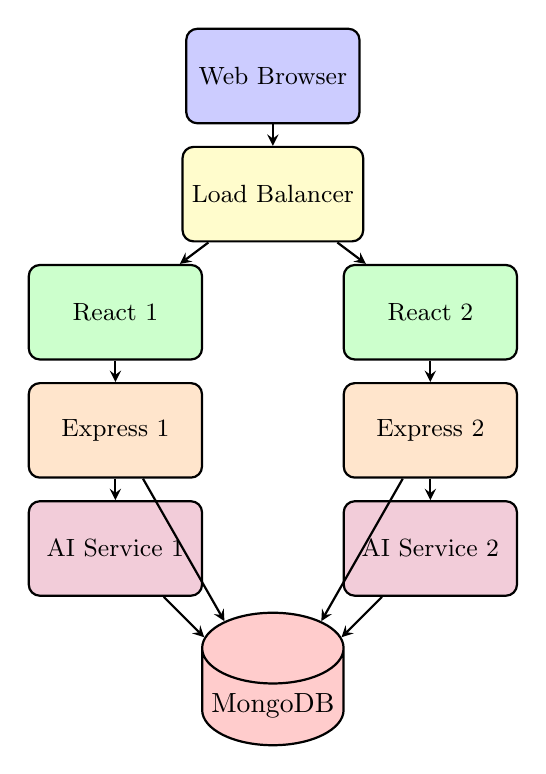
\begin{tikzpicture}[
    server/.style={rectangle, draw=black, thick, minimum width=2.2cm, minimum height=1.2cm, text centered, rounded corners, font=\small},
    database/.style={cylinder, draw=black, thick, minimum width=1.5cm, minimum height=1.5cm, shape border rotate=90, aspect=0.5},
    arrow/.style={->, >=stealth, thick, font=\tiny}
]

% Client Layer
\node[server, fill=blue!20] (client) at (0,5) {Web Browser};

% Load Balancer
\node[server, fill=yellow!20] (lb) at (0,3.5) {Load Balancer};

% Frontend Servers
\node[server, fill=green!20] (react1) at (-2,2) {React 1};
\node[server, fill=green!20] (react2) at (2,2) {React 2};

% Backend Servers
\node[server, fill=orange!20] (express1) at (-2,0.5) {Express 1};
\node[server, fill=orange!20] (express2) at (2,0.5) {Express 2};

% AI Microservice
\node[server, fill=purple!20] (ai1) at (-2,-1) {AI Service 1};
\node[server, fill=purple!20] (ai2) at (2,-1) {AI Service 2};

% Databases
\node[database, fill=red!20] (mongodb) at (0,-3) {MongoDB};

% Connections
\draw[arrow] (client) -- (lb);
\draw[arrow] (lb) -- (react1);
\draw[arrow] (lb) -- (react2);
\draw[arrow] (react1) -- (express1);
\draw[arrow] (react2) -- (express2);
\draw[arrow] (express1) -- (ai1);
\draw[arrow] (express2) -- (ai2);
\draw[arrow] (express1) -- (mongodb);
\draw[arrow] (express2) -- (mongodb);
\draw[arrow] (ai1) -- (mongodb);
\draw[arrow] (ai2) -- (mongodb);

\end{tikzpicture}%
}
\caption{Deployment Architecture Diagram}
\label{fig:deployment}
\end{figure}

\section{Data Flow Diagram}
Figure~\ref{fig:dataflow} shows the data flow for the symptom checking process.

\begin{figure}[H]
\centering
\resizebox{0.95\textwidth}{!}{%
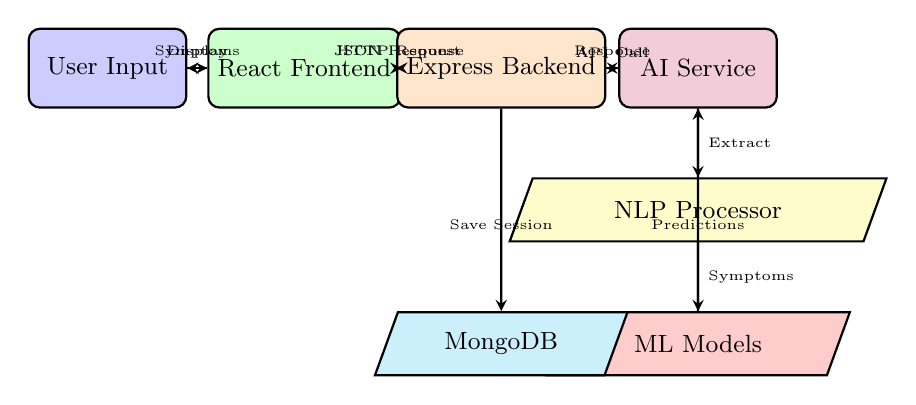
\begin{tikzpicture}[
    process/.style={rectangle, draw=black, thick, minimum width=2cm, minimum height=1cm, text centered, rounded corners, font=\small},
    data/.style={trapezium, draw=black, thick, minimum width=1.8cm, minimum height=0.8cm, text centered, trapezium left angle=70, trapezium right angle=110, font=\small},
    arrow/.style={->, >=stealth, thick, font=\tiny}
]

\node[process, fill=blue!20] (user) at (0,0) {User Input};
\node[process, fill=green!20] (frontend) at (2.5,0) {React Frontend};
\node[process, fill=orange!20] (backend) at (5,0) {Express Backend};
\node[process, fill=purple!20] (ai) at (7.5,0) {AI Service};
\node[data, fill=yellow!20] (nlp) at (7.5,-1.8) {NLP Processor};
\node[data, fill=red!20] (ml) at (7.5,-3.5) {ML Models};
\node[data, fill=cyan!20] (db) at (5,-3.5) {MongoDB};

\draw[arrow] (user) -- node[above, font=\tiny] {Symptoms} (frontend);
\draw[arrow] (frontend) -- node[above, font=\tiny] {HTTP Request} (backend);
\draw[arrow] (backend) -- node[above, font=\tiny] {API Call} (ai);
\draw[arrow] (ai) -- node[right, font=\tiny] {Extract} (nlp);
\draw[arrow] (nlp) -- node[right, font=\tiny] {Symptoms} (ml);
\draw[arrow] (ml) -- node[below, font=\tiny] {Predictions} (ai);
\draw[arrow] (ai) -- node[above, font=\tiny] {Response} (backend);
\draw[arrow] (backend) -- node[below, font=\tiny] {Save Session} (db);
\draw[arrow] (backend) -- node[above, font=\tiny] {JSON Response} (frontend);
\draw[arrow] (frontend) -- node[above, font=\tiny] {Display} (user);

\end{tikzpicture}%
}
\caption{Data Flow Diagram for Symptom Checking}
\label{fig:dataflow}
\end{figure}

\section{Component Interaction Diagram}
Figure~\ref{fig:component} shows the component interaction for the complete MERN application.

\begin{figure}[H]
\centering
\resizebox{0.9\textwidth}{!}{%
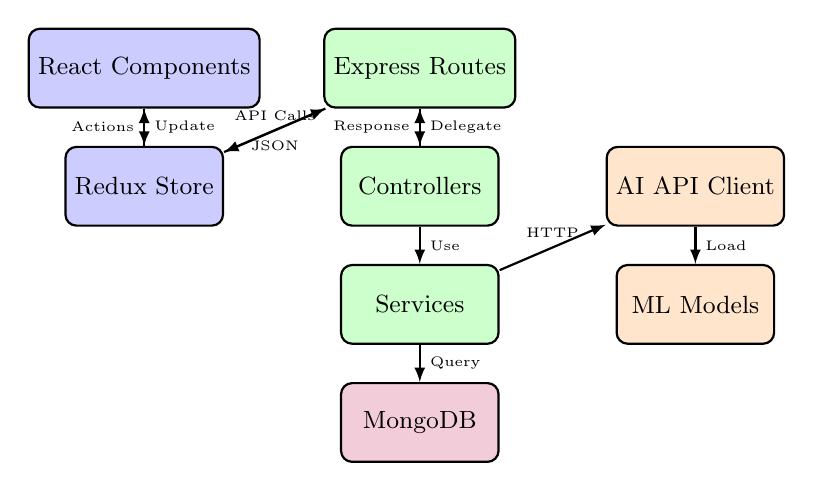
\begin{tikzpicture}[
    component/.style={rectangle, draw=black, thick, minimum width=2cm, minimum height=1cm, text centered, rounded corners, font=\small},
    arrow/.style={->, >=stealth, thick, >=latex, font=\tiny}
]

% Frontend Components
\node[component, fill=blue!20] (react) at (-3.5,3) {React Components};
\node[component, fill=blue!20] (redux) at (-3.5,1.5) {Redux Store};

% Backend Components
\node[component, fill=green!20] (routes) at (0,3) {Express Routes};
\node[component, fill=green!20] (controllers) at (0,1.5) {Controllers};
\node[component, fill=green!20] (services) at (0,0) {Services};

% AI Components
\node[component, fill=orange!20] (aiapi) at (3.5,1.5) {AI API Client};
\node[component, fill=orange!20] (aimodels) at (3.5,0) {ML Models};

% Database
\node[component, fill=purple!20] (db) at (0,-1.5) {MongoDB};

% Connections
\draw[arrow] (react) -- node[left, font=\tiny] {Actions} (redux);
\draw[arrow] (redux) -- node[above, font=\tiny] {API Calls} (routes);
\draw[arrow] (routes) -- node[right, font=\tiny] {Delegate} (controllers);
\draw[arrow] (controllers) -- node[right, font=\tiny] {Use} (services);
\draw[arrow] (services) -- node[above, font=\tiny] {HTTP} (aiapi);
\draw[arrow] (aiapi) -- node[right, font=\tiny] {Load} (aimodels);
\draw[arrow] (services) -- node[right, font=\tiny] {Query} (db);
\draw[arrow] (controllers) -- node[left, font=\tiny] {Response} (routes);
\draw[arrow] (routes) -- node[below, font=\tiny] {JSON} (redux);
\draw[arrow] (redux) -- node[right, font=\tiny] {Update} (react);

\end{tikzpicture}%
}
\caption{Component Interaction Diagram}
\label{fig:component}
\end{figure}

\section{Medical Disclaimer}
\textbf{IMPORTANT}: This system is for informational purposes only and does not provide medical advice, diagnosis, or treatment. Always consult qualified healthcare professionals for medical concerns. The system should not be used as a substitute for professional medical care, especially in emergency situations.

\end{document}
